%% IEEE TAES manuscript (official IEEEtaes.cls + IEEEtaes.bst, both in this dir).
%% Build: pdflatex -> bibtex -> pdflatex x2.
%% Citation integrity: python check_citations.py . --no-net
\documentclass{IEEEtaes}

\usepackage{amsmath,amssymb,amsfonts}
\usepackage{graphicx}
\usepackage{booktabs}
\usepackage{array}
\usepackage{siunitx}
% IEEEtaes.cls already loads hyperref; only adjust its options here.
\hypersetup{hidelinks}
\usepackage{algorithm}
\usepackage{algpseudocode}
\usepackage{pifont}

\jvol{XX}
\jnum{XX}
\jmonth{XXXXX}
\paper{1234567}
\pubyear{2026}
\doiinfo{TAES.2026.Doi Number}

\newtheorem{proposition}{Proposition}
\newtheorem{corollary}{Corollary}
\newtheorem{lemma}{Lemma}
\newtheorem{definition}{Definition}
\newtheorem{assumption}{Assumption}
\newtheorem{remark}{Remark}
\newtheorem{problem}{Problem}

\begin{document}

\title{Joint Aeromagnetic Compensation and Magnetic-Anomaly Navigation with a Fixed-Lag Factor Graph}

\author{Jayden Dongwoo Lee}
\affil{Korea Advanced Institute of Science and Technology, Daejeon, Korea}

\author{Bohyun Chang}
\affil{Korea Advanced Institute of Science and Technology, Daejeon, Korea}

\author{Hyochoong Bang}
\member{Member, IEEE}
\affil{Korea Advanced Institute of Science and Technology, Daejeon, Korea}

\receiveddate{Manuscript received XXXXX 00, 0000; revised XXXXX 00, 0000; accepted XXXXX 00, 0000.}

\corresp{{\itshape (Corresponding author: H. Bang)}.}

\authoraddress{J. D. Lee, B. Chang, and H. Bang are with the Department of Aerospace Engineering, Korea Advanced Institute of Science and Technology, Daejeon 34141, Republic of Korea (e-mail: \href{mailto:cin6474@kaist.ac.kr}{cin6474@kaist.ac.kr}; \href{mailto:hcbang@kaist.ac.kr}{hcbang@kaist.ac.kr}).}

\editor{}
\supplementary{}

\markboth{LEE ET AL.}{JOINT AEROMAGNETIC COMPENSATION AND MAGNETIC-ANOMALY NAVIGATION}
\maketitle

\begin{abstract}
Airborne magnetic-anomaly navigation bounds inertial drift in GNSS-denied flight
by matching a scalar magnetometer against a magnetic-anomaly map. Its central
obstacle is aeromagnetic interference: the aircraft's own field must be
compensated online when no calibration flight is available, the cold-start
regime. A recent approach augments an extended Kalman filter (EKF) with online
Tolles--Lawson (TL) coefficients and a residual neural network. We instead cast
navigation and compensation as one maximum-a-posteriori problem on a factor graph,
carrying the TL coefficients as time-varying graph variables so the compensation
adapts along the flight with no neural network. That single problem is solved
across a spectrum of lags under one cost function: a full-line batch that sets the
offline accuracy bound, a fixed-lag sliding window, and a per-epoch incremental
smoother that reaches the real-time limit at \SI{7.8}{\milli\second} per state. The
lag is the primary design variable, trading the future data that corrects a committed
state against latency. A linear condition states when position can be separated
from compensation and predicts a cold-start transient that the experiments
decompose into a warm-prior part and a map-observability part. Across cold-start
lines from two flights and two maps, the smoother is the most accurate of four
estimators on every full-length case (\num{8} of \num{8}), and on six of the eight
with its look-ahead removed entirely: it stays bounded where an
online-TL EKF diverges and a marginalized particle filter is erratic, and, carrying no
learned component of its own, it beats a tuned EKF+TL+NN baseline. At the shortest
lag the compensation prior decides the cold start. One scalar standard deviation
shared by a regressor whose columns span four orders of magnitude leaves the
first linearizations stiff in the compensation relative to position, so roughly
\SI{2000}{\nano\tesla} of uncompensated cabin field is charged to position
through the map gradient and the estimate leaves the map. No lag, robust kernel,
map resolution, relinearization schedule, measurement rate, process-noise floor,
or single choice of measurement-noise scale repairs it; raising that one
standard deviation by two orders of magnitude removes it on every affected
line. A Monte-Carlo simulation confirms
the reported covariance is consistent, and an independent GTSAM reimplementation
sharing no code reproduces the bounded result to within a metre on both
magnetometers once the compensation cold start is handled.
\end{abstract}

\begin{IEEEkeywords}
Magnetic-anomaly navigation, aeromagnetic compensation, Tolles--Lawson,
factor-graph optimization, fixed-lag smoothing, GNSS-denied navigation.
\end{IEEEkeywords}

\section*{Nomenclature}
\addcontentsline{toc}{section}{Nomenclature}
\begin{IEEEdescription}[\IEEEsetlabelwidth{$\boldsymbol{\Phi}_t,\mathbf{Q}_t$}]
\item[$\mathbf{x}_t$] INS error state at epoch $t$ (position, velocity, attitude,
baro-inertial pair, IMU biases, FOGM), $\mathbf{x}_t\in\mathbb{R}^{18}$.
\item[$\boldsymbol{\beta}_t$] Online Tolles--Lawson compensation coefficients.
\item[$\boldsymbol{\chi}_t$] Joint state $(\mathbf{x}_t,\boldsymbol{\beta}_t)$.
\item[$\boldsymbol{\Phi}_t,\mathbf{Q}_t$] Pinson state-transition matrix and process
covariance.
\item[$z_t,\,\eta_t$] Scalar magnetometer measurement and its noise, variance $R$.
\item[$h(\cdot)$] Anomaly-map interpolation (with IGRF core) as a function of
position.
\item[$\mathbf{g}_t$] Map gradient $\partial h/\partial\mathbf{p}$ at epoch $t$.
\item[$\mathbf{A}_t$] Tolles--Lawson basis row from the three-axis fluxgate.
\item[$c_t$] Aircraft magnetic interference, $c_t=\mathbf{A}_t^{\top}\boldsymbol{\beta}_t$.
\item[$L_w,\,L_o$] Sliding-window length and overlap (look-ahead).
\item[$\rho,\,\delta$] Robust kernel and its Huber threshold.
\item[$\mathbf{G},\boldsymbol{\Psi}$] Stacked map-gradient and TL-regressor matrices
over a window.
\item[$\mathcal{N}(\cdot,\cdot)$] Gaussian density.
\item[$\lVert\cdot\rVert_{\mathbf{M}}$] Mahalanobis norm,
$\lVert\mathbf{v}\rVert^2_{\mathbf{M}}=\mathbf{v}^{\top}\mathbf{M}\mathbf{v}$.
\end{IEEEdescription}

\noindent Boldface lowercase denotes vectors and boldface uppercase matrices.

\section{Introduction}

% P1: Big Picture
\IEEEPARstart{I}{nertial} navigation systems (INS) are the backbone of airborne
navigation, but their position error grows without bound as accelerometer and
gyroscope errors are integrated over time, so an INS must be aided by an absolute
position reference~\cite{groves2013,titterton2004}. The satellite-based reference
of choice, GNSS, is unavailable or untrustworthy in the contested and
signal-degraded environments that increasingly define aerospace and defense
operations. This has renewed interest in passive, self-contained references that
draw on natural geophysical signatures of the Earth. Among these, the crustal
magnetic-anomaly field is attractive: it is globally available, temporally stable
over the mission horizon, and observable with a lightweight scalar
magnetometer~\cite{canciani2016,canciani2017}. It is also difficult to spoof from a
stand-off distance.
Denial of a satellite signal exploits the far-field radio link, whose power falls
off only as the inverse square of range, so a modest transmitter jams or spoofs a
receiver from far away; a magnetic anomaly, by contrast, is a near-field source
whose dipole field decays as the inverse cube of distance, so counterfeiting a
credible anomaly at a moving aircraft would demand an impractically large or close
field source~\cite{qctrl2025}. % (IEEE Xplore 11079836) once its metadata is supplied
The same map-matching idea underlies
terrain-referenced and gravity-referenced navigation, where an onboard measurement
is matched against a stored geophysical map to bound inertial
drift~\cite{golden1980,hostetler1983,nordlund2009}; magnetic-anomaly navigation is
distinguished by the ubiquity and fine spatial structure of the crustal field and by
the maturity of airborne magnetic surveying. These properties make it a candidate
absolute reference for long-endurance aircraft, uncrewed platforms, and
munitions operating where GNSS cannot be trusted, provided the aircraft's own
magnetic signature can be removed in flight.

\begin{figure*}[t]
\centering
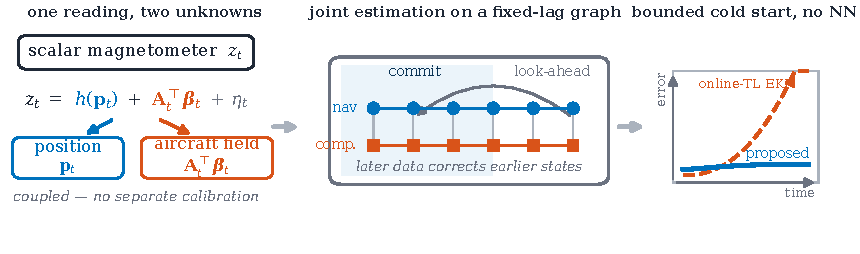
\includegraphics[width=0.98\textwidth]{figs/fig_concept.pdf}
\caption{Concept of the study: (a)~one scalar reading couples aircraft position and
aircraft-field compensation; (b)~a fixed-lag factor graph estimates both jointly,
letting later measurements correct earlier states; (c)~bounded cold-start
navigation, with no neural network.}
\label{fig:concept}
\end{figure*}

% P2a: Maturity of the field, and the two distinct deployment obstacles
Magnetic-anomaly navigation (MagNav) estimates aircraft position by matching the
measured scalar field against a surveyed anomaly map, yielding an absolute fix that
bounds inertial drift~\cite{canciani2017}. The idea has matured from feasibility
study to flight demonstration: recursive Bayesian map matching, from the extended
Kalman filter to grid and particle estimators, was characterized on flight
data~\cite{canciani2016,canciani2017} and flown on an F-16~\cite{canciani2020}, and
recent multi-hour fixed-wing trials over thousands of kilometres report
metre-to-decametre accuracy with quantum magnetometers~\cite{qctrl2025}. As the
estimators have matured, attention has moved to the inputs they rely on, and a
consensus is forming that the pacing requirement for operational deployment is a
sufficiently accurate, uncertainty-aware anomaly map~\cite{angappan2026}. Two
obstacles, in fact, separate these demonstrations from routine use, and they are
distinct: the reference map on the ground and the aircraft's own field in the air.
The map is a survey-and-data problem, pursued elsewhere~\cite{angappan2026}; this
paper addresses the second.

% P2b: The aircraft-field compensation problem
The platform's own permanent and induced magnetization and its eddy-current fields
perturb the scalar measurement by hundreds of nanotesla, comparable to or larger
than the anomaly signal being matched, so the aircraft field must be compensated
before map matching can recover position. This aircraft-field problem is intrinsic
to MagNav and independent of any particular airframe; it is most acute for
magnetometers mounted inside the cabin, close to avionics and current-carrying
structure, rather than on a wingtip stinger boom that holds the sensor away from the
platform field.

% P3: Technical Background -- two orthogonal difficulties, mostly attacked offline
Aeromagnetic compensation is classically handled by the Tolles--Lawson (TL)
model~\cite{tolles1950,leliak1961,bickel1979}, a regression of the interference onto
sixteen attitude-dependent terms (permanent, induced, and eddy-current) formed from a
three-axis fluxgate magnetometer. It faces two difficulties that are easy to conflate
but are in fact orthogonal. The first is temporal: the coefficients are
conventionally identified on a dedicated high-altitude calibration flight of
prescribed maneuvers, yet many operational scenarios admit none, and the coefficients
drift with temperature and configuration. In this cold-start regime they must be
estimated online and jointly with navigation, from the same measurements that fix
position, a coupling that makes both estimation and its analysis substantially harder
than the calibrated case. The second is representational: however well its
coefficients are fit, the linear TL basis cannot span interference from platform
currents and other non-rigid, non-attitude sources, which contribute a large fraction
of the field on cabin-mounted sensors~\cite{gnadt2020,gnadt2022}. One difficulty is
about identifying a known model class in time; the other is about that class being
too small.

A public benchmark has made both concrete: the Signal Enhancement for Magnetic
Navigation (SGL~2020) challenge dataset~\cite{gnadt2020}, with flight-grade INS,
wingtip-stinger and cabin-mounted magnetometers, and high-resolution anomaly maps.
Most work on it attacks the two difficulties offline: the TL coefficients by a
batch calibration flight, and the representational gap by learned models fit offline
on logged data, neural-network heading-error and denoising
compensators~\cite{williams1993,gnadt2022}, physics-informed liquid-time-constant
networks~\cite{nerrise2024}, and model-stability studies of the regression in
gradiometry~\cite{noriega2015}. Offline learning, however, presupposes exactly
what the operational scenario lacks: a corpus of logged flights from the same
aircraft, a reference-grade compensated sensor flying alongside to supply training
targets, the computation to train on that corpus, and a willingness to retrain
whenever the platform configuration or its magnetic state drifts. A compensator
fit this way is specific to one airframe in one equipment state, and its accuracy
in flight is bounded by how well the training corpus transfers to the day's
conditions. We therefore treat the offline family as context rather than
competition: every estimator compared in this paper starts, as ours does, from no
prior flight data. The exception is the online NN-in-EKF line of work
originated by Gnadt~\cite{gnadt2022}, which carries the TL coefficients and the
weights of a residual network as filter states learned in flight, and which has
recently been extended with an error-state formulation and a natural-gradient
interpretation~\cite{hager2026}; this lineage holds, to our knowledge, the
strongest reported cold-start results on the benchmark. This paper takes on the
temporal difficulty fully: online, joint estimation of a time-varying
compensation. The representational gap it does not model term-by-term: instead of a
learned remainder, the estimator absorbs what the TL basis misses structurally,
through the time-varying coefficients, a colored disturbance state, and a robust
kernel, and Section~\ref{sec:results} verifies against the recorded platform
currents how much of the remainder this accounts for.

% P4: Cluster A -- Bayesian filtering / map matching
Recursive Bayesian filtering is the standard machinery for map-matching
navigation, from the linear Kalman filter~\cite{kalman1960} to nonlinear variants.
Geophysical map matching has a long lineage: terrain-contour matching for cruise
missiles~\cite{golden1980} and nonlinear Kalman filtering for terrain-aided
navigation~\cite{hostetler1983} established the paradigm, and grid- and
particle-based Bayesian estimators later became standard where the
measurement-to-position map is strongly nonlinear or
multimodal~\cite{bergman1999,gustafsson2002,anonsen2006,nordlund2009}. For MagNav
specifically, Canciani and Raquet combined a calibrated scalar magnetometer with an
extended Kalman filter (EKF) and characterized the achievable accuracy on flight
data~\cite{canciani2016,canciani2017}, later demonstrating airborne magnetic
navigation with online calibration~\cite{canciani2020}. Beyond the EKF, unscented
filtering~\cite{julier2004}, invariant formulations that respect the state
manifold~\cite{barrau2017}, and mixture/particle representations~\cite{barshalom2001}
improve consistency under nonlinearity. However, these estimators are causal:
they commit each state online with no access to future measurements, and the
position-centric ones carry no compensation state of their own. When a large
uncompensated cold-start residual enters, a causal filter has no mechanism to
attribute the mismatch to the aircraft field rather than to position, and, unable to
revise a committed state, the estimate can diverge.

% P5: Cluster B -- online / learned compensation
A second line of work makes the compensation itself adaptive. Classical
Tolles--Lawson (TL) identification is a batch regression on a calibration
flight~\cite{tolles1950,leliak1961,bickel1979}; to remove that requirement the TL
regression can be embedded in the estimator and its coefficients tracked online as
additional states. Nonlinear extensions replace or augment the linear basis with
learned components: neural-network compensators date back three
decades~\cite{williams1993}, model-stability and robustness of the regression have
been studied in gradiometry~\cite{noriega2015}, and machine-learning-enhanced
calibration has recently been applied to the SGL benchmark~\cite{gnadt2022}. Most
relevant here, a residual neural network (NN) has been added on top of an online TL
model, carried inside an EKF and trained online, to capture interference the linear
basis misses, introduced with Gnadt's online models~\cite{gnadt2022} and recently
extended in~\cite{hager2026}; this reaches good cold-start accuracy on the SGL~2020
cabin magnetometers and holds, to our knowledge, the strongest reported cold-start
results on that benchmark. Nevertheless, the network requires a carefully
engineered online-training design to remain stable, adds opaque parameters whose
behavior is hard to certify, and, being embedded in an EKF, inherits the same
causal, commit-online limitation as the filters above.

% P6: Cluster C -- factor-graph smoothing
A third body of work, largely from robotics, replaces filtering with factor-graph
optimization: the estimation problem is a graph of variables and probabilistic
constraints~\cite{kschischang2001} whose maximum-a-posteriori (MAP) solution is
found by sparse nonlinear least squares~\cite{dellaert2017,dellaert2012}, the same
structure underlying bundle adjustment and graph SLAM~\cite{triggs2000,grisetti2010,kummerle2011}.
Incremental and square-root smoothers (square-root
SAM~\cite{dellaert2006}, iSAM~\cite{kaess2008}, iSAM2~\cite{kaess2012}, and
exactly-sparse delayed-state filters~\cite{eustice2006}) make the solution
efficient enough for online use, and fixed-lag sliding-window
optimization~\cite{sibley2010,leutenegger2015} bounds its cost. On-manifold inertial
preintegration~\cite{forster2017}, factor-graph inertial
fusion~\cite{indelman2013}, and modern visual--inertial estimators~\cite{qin2018}
have brought the approach firmly into navigation. Despite these advances,
factor-graph estimation in navigation has been developed almost entirely for
visual--inertial odometry and simultaneous localization and mapping, where the
estimated quantities are poses and landmarks. The factor graph has very recently
reached aeromagnetic compensation itself: Lathrop et al.~\cite{lathrop2024}
calibrate a magnetometer by fusing vector and scalar magnetometers with inertial
measurements in a factor graph, absorbing large permanent moments and a
time-varying external field. That work compensates the sensor but does not close
the loop to navigation. The joint problem, estimating a time-varying compensation
together with aircraft position from map matching, has not, to our knowledge, been
posed in a published factor-graph formulation, and the observability of doing so has
not been characterized.

% P6.5: Synthesis of the gap
Taken together, the three lines leave a specific gap. The cold-start MagNav problem
is fundamentally a joint estimation of position and a time-varying
compensation model from a single scalar stream, in which the two unknowns are
confounded through the very measurement that must resolve them. Causal filters
(cluster~A) must commit each state before the maneuvers that would disambiguate the
compensation have occurred, and so diverge when the initial residual is large;
learned online compensation (cluster~B) repairs that residual but keeps the causal,
commit-online architecture and adds parameters that are difficult to certify; and
factor-graph smoothing (cluster~C), which can defer commitment and estimate
structured nuisance variables jointly, has not been applied to this problem, nor has
anyone characterized when the joint problem is even observable. What is missing is
an estimator that (i)~defers commitment so that late-arriving calibration
information corrects early navigation states, (ii)~represents the compensation as
first-class, time-varying variables rather than a black box, and (iii)~comes with
an explicit condition for when position and compensation can be separated at all.
This paper supplies all three.

% P7: Proposed approach + contributions
In this work we cast magnetic-anomaly navigation as a factor graph and, within it,
carry the online Tolles--Lawson coefficients as time-varying variables, so that
navigation and compensation are solved jointly as one maximum-a-posteriori (MAP)
problem (Fig.~\ref{fig:concept}). Rather than fix a single filter or smoother, we
solve that one problem across a spectrum of lags: a full-line batch that uses every
measurement and sets the offline accuracy bound, a fixed-lag sliding window that
commits a state once it has seen a bounded amount of future data, and a per-epoch
incremental smoother, built on iSAM2~\cite{kaess2012}, that takes the lag to its
real-time limit. The lag is the primary design variable along this spectrum, trading
observability, the amount of future data that corrects a committed state, against latency and
computation. What unites every point on it, and separates all of them from the causal
filters of clusters~A and~B, is that each committed state can be relinearized and
revised as later measurements arrive, so late calibration corrects early navigation;
a causal filter commits each state once and cannot revise it. We are explicit about
scope: for the linear--Gaussian INS error model the batch MAP estimate on the
factor-graph chain equals the Rauch--Tung--Striebel (RTS) smoother~\cite{rauch1965},
so smoothing per se is not the contribution; the joint estimation of a time-varying
compensation, realized across the lag spectrum, is.
The paper makes the following contributions:
\begin{enumerate}
  \item \textbf{Factor-graph joint compensation.} We carry the online
        Tolles--Lawson coefficients as time-varying variables of a factor graph so
        that navigation and compensation are estimated jointly from the same scalar
        measurements. To the authors' knowledge this is the first factor-graph
        formulation that jointly estimates time-varying Tolles--Lawson compensation
        coefficients and navigation states in the calibration-cold-start regime.
        Relinearizing the coefficients as the graph is re-solved makes the
        compensation adapt along the flight, the role a learned online model plays in
        the competing filter, while the graph keeps every quantity an explicit,
        physically interpretable state.
  \item \textbf{A MAP estimation spectrum.} We solve that one MAP problem across a
        spectrum of lags under a single cost function: an offline full-line batch, a
        fixed-lag sliding window, and a per-epoch incremental smoother built on
        iSAM2. The lag is the primary design variable trading observability against
        latency and computation, so the batch fixes the offline accuracy bound and
        the incremental smoother runs in real time
        (\SIrange{6.0}{9.0}{\milli\second} per state at a \SI{300}{\second} lag and
        \SI{1}{\hertz} states, two orders of magnitude within the state cadence).
        This places recursive filtering and batch smoothing as two limits of
        one estimator rather than competing methods, and every point on the spectrum
        can re-smooth the past, the property the cold start needs.
  \item \textbf{Position--compensation separability and the cold-start transient.}
        We give a linear-algebraic condition, evaluated over a window, for when a
        position error can be distinguished from a change in the compensation, separating
        three failure modes: an unexcited trajectory, a rank-deficient compensation
        basis, and the subtle one, a compensation subspace aligned with the anomaly
        gradient. The condition predicts the cold-start transient, which the
        experiments decompose: a warm compensation prior cuts it by \SI{40}{\percent}, and the remaining
        transient tracks map-gradient observability rather than compensation error.
        Separately, and ahead of any observability question, we identify the
        setting that decides whether a short-lag smoother survives a cold start at
        all: the scale of the compensation prior relative to the regressor. We
        measure the failure, rule out the lag, the robust kernel, the map
        resolution, the relinearization schedule, the measurement rate, the
        measurement-noise scale and the process-noise floor as causes, and show
        that raising the compensation prior by two orders of magnitude, or setting it
        per regressor column, removes it on every affected line.
  \item \textbf{Flight-data validation.} On uncompensated cabin magnetometers across
        eight cold-start cases spanning four lines, two flights, and two maps, the
        smoother is the most accurate of four cold-start estimators. Run rather than
        merely cited, the online EKF+TL+NN lineage of~\cite{gnadt2022,hager2026} is
        kept bounded by its network where a weak online-TL EKF diverges and a
        marginalized particle filter is erratic, yet the smoother beats it with no
        learned component. A Monte-Carlo simulation confirms the reported covariance
        is consistent, and an independent GTSAM reimplementation~\cite{dellaert2012}
        that shares no code reproduces the bounded cold-start result, separating the
        estimator from its implementation.
\end{enumerate}

% P8: Organization
The remainder of this paper is organized as follows.
Section~\ref{sec:background} states the INS error model, the measurement, and the
batch MAP problem. Section~\ref{sec:method} develops the factor graph and solves it
across the lag spectrum, from the batch bound to the per-epoch incremental smoother.
Section~\ref{sec:observability}
establishes the separability condition. Section~\ref{sec:results} describes the
baselines and reports and
interprets the experiments. Section~\ref{sec:conclusion} concludes and states the
limitations.

\section{Problem Formulation}\label{sec:background}
The situation this paper addresses is the cold start: an aircraft departs with an
uncalibrated magnetometer installation, its INS error grows, and the only absolute
position information is a scalar magnetic reading in which the map signal and the
aircraft's own field are mixed. The estimation task is therefore joint from the
outset: there is no separate calibration step whose output a navigator could
consume:

\begin{problem}[Joint compensation and navigation]\label{prob:joint}
Given the scalar measurements $z_{1:N}$, the
fluxgate regressor rows $\mathbf{A}_{1:N}$, the
anomaly map $h$, the INS mechanization, and the
prior $(\hat{\boldsymbol{\chi}}_0,\mathbf{P}_0)$, estimate the joint trajectory
$\boldsymbol{\chi}_{1:N}$ of navigation errors and compensation coefficients,
$\boldsymbol{\chi}_t=(\mathbf{x}_t,\boldsymbol{\beta}_t)$.
\end{problem}

The rest of the section supplies the three models that make
Problem~\ref{prob:joint} concrete: how the navigation error evolves, what the scalar magnetometer measures, and how the aircraft field enters it. Section~\ref{sec:method} then casts the joint estimation as maximum-a-posteriori inference on a factor graph and solves it across a spectrum of lags.

\begin{figure*}[t]
\centering
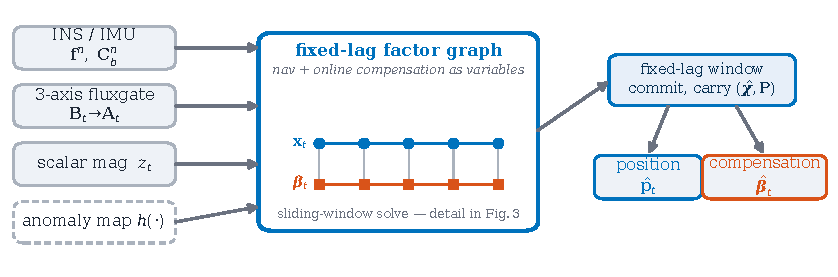
\includegraphics[width=0.92\textwidth]{figs/fig_pipeline.pdf}
\caption{Proposed estimator: the sensors feed a factor graph of navigation,
online TL compensation, solved over a
fixed-lag window.}
\label{fig:pipeline}
\end{figure*}

\subsection{INS error state and dynamics}
We adopt the standard Pinson error model of a strapdown INS~\cite{groves2013,titterton2004,farrell2008}.
The error state
\begin{equation}
\mathbf{x}=\big[\,\delta\mathbf{p}^{\top}\;\delta\mathbf{v}^{\top}\;
\boldsymbol{\psi}^{\top}\;h_a\;\hat{a}\;\mathbf{b}_a^{\top}\;\mathbf{b}_g^{\top}\;S\,\big]^{\top}
\in\mathbb{R}^{18}
\label{eq:state}
\end{equation}
stacks position error $\delta\mathbf{p}$, velocity error $\delta\mathbf{v}$,
attitude error $\boldsymbol{\psi}$ (three components each), the baro-inertial
altitude-aiding pair $(h_a,\hat{a})$ that damps the vertically unstable channel,
accelerometer and gyroscope biases $\mathbf{b}_a,\mathbf{b}_g$, and a scalar
first-order Gauss--Markov (FOGM) state $S$ that absorbs residual magnetic
disturbance and map error. The discretized,
linearized dynamics are
\begin{equation}
\mathbf{x}_{t+1}=\boldsymbol{\Phi}_t\mathbf{x}_t+\mathbf{w}_t,\qquad
\mathbf{w}_t\sim\mathcal{N}(\mathbf{0},\mathbf{Q}_t),
\label{eq:dyn}
\end{equation}
where $\boldsymbol{\Phi}_t$ is the Pinson state-transition matrix
(Appendix~\ref{app:pinson}) and
$\mathbf{Q}_t$ the process covariance; the FOGM block of $\boldsymbol{\Phi}_t$ is
$e^{-\Delta t/\tau}$ with correlation time $\tau$.

\subsection{Scalar magnetometer measurement}
The scalar magnetometer reads
\begin{equation}
z_t = h(\mathbf{p}_t) + c_t + \eta_t, \qquad \eta_t\sim\mathcal{N}(0,R),
\label{eq:meas}
\end{equation}
where $h(\cdot)$ interpolates the crustal anomaly map (with the IGRF core field
restored) at the aircraft position $\mathbf{p}_t=\bar{\mathbf{p}}_t+\delta\mathbf{p}_t$
and $c_t$ is the Tolles--Lawson part of the aircraft interference; the
non-Tolles--Lawson remainder is carried by the first-order Gauss--Markov state
$S_t$ introduced below. Linearizing about the nominal position,
\begin{equation}
z_t \approx h(\bar{\mathbf{p}}_t)+\mathbf{g}_t^{\top}\delta\mathbf{p}_t+c_t+\eta_t,
\qquad \mathbf{g}_t=\left.\frac{\partial h}{\partial\mathbf{p}}\right|_{\bar{\mathbf{p}}_t},
\label{eq:measlin}
\end{equation}
so the map gradient $\mathbf{g}_t$ is the sole source of horizontal position
information: where $\mathbf{g}_t\!\approx\!\mathbf{0}$ (a locally flat map) position
is momentarily unobservable, and everywhere the interference $c_t$ competes with the
$\mathbf{g}_t^{\top}\delta\mathbf{p}_t$ term for the same measurement. The map $h$ is
stored as a gridded anomaly product upward-continued to the survey altitude; we
evaluate it and its gradient by bicubic interpolation, which yields the continuous
$\mathbf{g}_t$ required to linearize~\eqref{eq:measlin}, and we restore the IGRF core
field so that $z_t$ and $h$ are on a common absolute scale. The gradient magnitude
$\lVert\mathbf{g}_t\rVert$ varies by more than an order of magnitude along a line,
which is why position accuracy is not uniform in time even for a perfect
compensator, a point the error traces of Section~\ref{sec:results} make visible.

\subsection{Tolles--Lawson interference model}
Classical aeromagnetic compensation writes the interference as a linear combination
of attitude-dependent basis terms~\cite{tolles1950,leliak1961,bickel1979},
\begin{equation}
c_t=\mathbf{A}_t^{\top}\boldsymbol{\beta}_t,
\label{eq:tl}
\end{equation}
where $\mathbf{A}_t\in\mathbb{R}^{m}$ is the TL basis row of~\eqref{eq:tl} built
from the three-axis fluxgate; its classical rank deficiency is a gauge freedom
(Remark~\ref{rem:gauge}). With direction cosines $\hat{\mathbf{b}}_t=[\,u\;v\;w\,]^{\top}$ of the
Earth field in body axes and total field magnitude $B_t$, the permanent (3),
induced (6), and eddy-current (9) groups are
\begin{equation}
\mathbf{A}_t=\big[\underbrace{u,v,w}_{\text{perm.}},\;
\underbrace{B_tu^2,\dots,B_tw^2}_{\text{induced}},\;
\underbrace{B_tu\dot u,\dots,B_tw\dot w}_{\text{eddy}}\big]^{\top},
\label{eq:tlbasis}
\end{equation}
optionally augmented by a bias term, giving $m\!\le\!19$ coefficients
$\boldsymbol{\beta}_t$. In the calibrated setting $\boldsymbol{\beta}$ is fit once
and frozen; in the cold-start setting it is unknown at takeoff and drifts slowly, so
we treat it as a time-varying state with a random-walk prior
$\boldsymbol{\beta}_{t+1}=\boldsymbol{\beta}_t+\mathbf{w}^{\beta}_t$,
$\mathbf{w}^{\beta}_t\sim\mathcal{N}(\mathbf{0},\mathbf{Q}^{\beta})$.

\section{MAP Estimation Spectrum}\label{sec:method}
Problem~\ref{prob:joint} has a single maximum-a-posteriori solution; what a designer
chooses is how much of the flight to weigh before committing an estimate. Solving it
over a lag of $L$ epochs traces a spectrum under one cost function: the full-line
batch ($L=N$) uses every measurement and is the offline accuracy bound; a per-epoch
recursion (small $L$) commits each state as soon as it is measured, for real-time
use; and the fixed-lag sliding window sits in between, committing a state once it has
seen a bounded amount of future data. The lag is thus the primary design variable that
trades observability, through the future data each committed estimate sees, against
latency and computation, and every point on the spectrum solves the same factor
graph. This section develops that graph and its batch solution, then the fixed-lag
window, then the per-epoch incremental smoother that is the window's real-time limit,
and finally the robust kernel and sparse solver common to all three; the estimator is
drawn in Fig.~\ref{fig:pipeline}, and the three realizations of the spectrum are
sketched in Fig.~\ref{fig:spectrum}.

\begin{figure}[t]
\centering
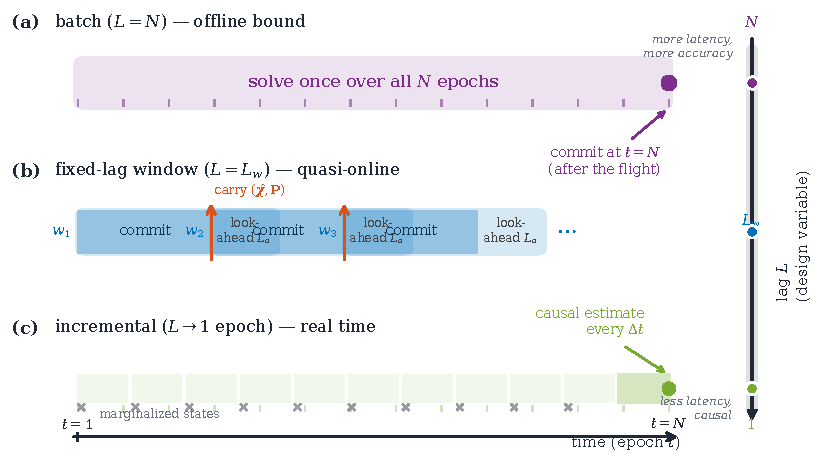
\includegraphics[width=\columnwidth]{figs/fig_spectrum.pdf}
\caption{The MAP estimation spectrum: the same factor graph solved at three lags,
from the full-line batch bound through the fixed-lag window to the per-epoch
incremental smoother, trading the future data each committed estimate sees against
latency.}
\label{fig:spectrum}
\end{figure}

\subsection{Batch MAP estimation (offline bound)}
The three models of Section~\ref{sec:background} couple through a single scalar
stream: the same measurement $z_t$
must simultaneously fix position through the map term $h(\mathbf{p}_t)$ and
identify the compensation $\mathbf{A}_t^{\top}\boldsymbol{\beta}_t$. We take the
maximum-a-posteriori (MAP) estimate of Problem~\ref{prob:joint}. Because the
dynamics are Markov and each measurement depends only on the current state, the
posterior splits into one factor per piece of information: a prior, one dynamics
factor per step for each of the two chains, and one measurement factor per epoch,
{\setlength{\abovedisplayskip}{2pt}\setlength{\abovedisplayshortskip}{2pt}%
\begin{equation}
\begin{aligned}
p(\boldsymbol{\chi}_{1:N}\mid z_{1:N})\;\propto\;
p(\boldsymbol{\chi}_1)
&\prod_{t=1}^{N-1} p(\mathbf{x}_{t+1}\mid\mathbf{x}_t)\,
p(\boldsymbol{\beta}_{t+1}\mid\boldsymbol{\beta}_t)\\[-2pt]
&\;\times\prod_{t=1}^{N} p(z_t\mid\boldsymbol{\chi}_t).
\end{aligned}
\label{eq:factorization}
\end{equation}}
This factorization is a factor graph~\cite{kschischang2001,dellaert2017}: a
bipartite graph whose variable nodes carry the unknowns and whose factor nodes carry
the individual densities in~\eqref{eq:factorization}, each edge joining a factor to
the variables it constrains (Fig.~\ref{fig:graph}). Concretely, there is one
variable node per epoch holding the joint state
$\boldsymbol{\chi}_t=(\mathbf{x}_t,\boldsymbol{\beta}_t)$, the $18$ Pinson error
states of~\eqref{eq:state} and the $m\!\le\!19$ TL coefficients
of~\eqref{eq:tlbasis}, so the graph has $N$ variable nodes and
$N\,(18{+}m)$ scalar unknowns. Four factor types populate it: a single unary
prior factor on $\boldsymbol{\chi}_1$; $N{-}1$ binary INS dynamics
factors, each linking $\mathbf{x}_t$ to $\mathbf{x}_{t+1}$
through~\eqref{eq:dyn}; $N{-}1$ binary compensation random-walk factors,
each linking $\boldsymbol{\beta}_t$ to $\boldsymbol{\beta}_{t+1}$; and $N$ unary
measurement factors, each attached to one node $\boldsymbol{\chi}_t$
through~\eqref{eq:meas}. The two dynamics families run as parallel chains that never
touch directly; the measurement factor is the only place position and compensation
meet, which is exactly why the two are estimated jointly and why their separability
needs a condition. MAP estimation on such a graph is sparse nonlinear
least squares: the negative logarithm of~\eqref{eq:factorization} turns each factor
into a squared or robust residual, and the Gauss--Newton normal equations
inherit the graph's chain sparsity, which is what makes batch solution tractable at
flight scale. Concretely, the MAP estimate minimizes
\begin{equation}
\begin{aligned}
J(\boldsymbol{\chi})=\;&\lVert\boldsymbol{\chi}_1-\boldsymbol{\chi}_0\rVert^2_{\mathbf{P}_0^{-1}}
+\sum_{t=1}^{N-1}\lVert\mathbf{x}_{t+1}-\boldsymbol{\Phi}_t\mathbf{x}_t\rVert^2_{\mathbf{Q}_t^{-1}}\\
&+\sum_{t=1}^{N-1}\lVert\boldsymbol{\beta}_{t+1}-\boldsymbol{\beta}_t\rVert^2_{(\mathbf{Q}^{\beta})^{-1}}
+\sum_{t=1}^{N}\rho\!\left(\frac{r_t(\boldsymbol{\chi}_t)}{\sqrt{R}}\right),
\end{aligned}
\label{eq:cost}
\end{equation}
Its four terms are, in order, the prior, the INS dynamics, the compensation
random walk, and the measurement misfit under a possibly robust kernel $\rho$;
the measurement residual $r_t(\boldsymbol{\chi}_t)$ of~\eqref{eq:resid} is what the
model cannot yet explain. The prior anchors both blocks of
$\boldsymbol{\chi}_1=(\mathbf{x}_1,\boldsymbol{\beta}_1)$. Its
$\boldsymbol{\beta}$-block $\mathbf{P}_0^{\beta}$ is the one setting a cold start
is sensitive to, because it decides how far the compensation may travel from zero
before the navigation states start absorbing the platform field; we return to it
in Section~\ref{sec:coldprior} and report its value in Table~\ref{tab:params}.
We make the standard modeling assumptions of aided inertial
navigation~\cite{groves2013,barshalom2001}.
\begin{assumption}\label{as:model}
The process and measurement noises $\mathbf{w}_t,\mathbf{w}^{\beta}_t,\eta_t$ are
zero-mean, white, mutually independent, and Gaussian; the linearizations
\eqref{eq:dyn} and \eqref{eq:measlin} are valid over a window; and the prior
$(\hat{\boldsymbol{\chi}}_0,\mathbf{P}_0)$ is Gaussian.
\end{assumption}
Assumption~\ref{as:model} is the same one under which the EKF and RTS smoother are
derived, so any performance difference between the estimators reflects their
structure, not their noise models. What Problem~\ref{prob:joint} adds over classical
map-matching is exactly the second chain: navigation and compensation are estimated
from the same evidence, and Section~\ref{sec:observability} characterizes when that
joint problem is well-posed.

With the compensation coefficients $\boldsymbol{\beta}$ carried as graph variables
throughout $\boldsymbol{\chi}_t$, the measurement factor of~\eqref{eq:meas} is, in
residual form,
\begin{equation}
r_t(\boldsymbol{\chi}_t)=z_t-h(\mathbf{p}_t)-\mathbf{A}_t^{\top}\boldsymbol{\beta}_t-S_t,
\label{eq:resid}
\end{equation}
with Gaussian information $R^{-1}$, and its Jacobian row is
\begin{equation}
\mathbf{H}_t=\Big[\underbrace{\mathbf{g}_t^{\top}}_{\delta\mathbf{p}}\;\;
\underbrace{\mathbf{0}}_{\delta\mathbf{v},\boldsymbol{\psi},h_a,\hat{a},\mathbf{b}}\;\;
\underbrace{\mathbf{A}_t^{\top}}_{\boldsymbol{\beta}}\;\;
\underbrace{1}_{S}\Big].
\label{eq:jac}
\end{equation}
These robust scalar-magnetometer factors, together with the Pinson--FOGM process
factors, the compensation random-walk factors, and the joint prior on
$\boldsymbol{\chi}_1$, form the four factor families of the graph in
Fig.~\ref{fig:graph}. The random-walk factor sets how quickly the coefficients may
adapt, with $\mathbf{Q}^{\beta}\!\to\!\mathbf{0}$ recovering a single static
$\boldsymbol{\beta}$ over the line.
The INS mechanization, the fluxgate (through $\mathbf{A}_t$), and the anomaly map
(through $h$ and $\mathbf{g}_t$) enter as known factor parameters, not as
estimated variables. Two
implementation details: in the online estimator only the horizontal components of
$\mathbf{g}_t$ are used (the vertical channel is baro-damped and the map is
evaluated at survey altitude), whereas the batch validation of
Section~\ref{sec:results}-A uses the full three-component gradient; and the
implementation orders the state vector as
$[\text{Pinson-17};\,\boldsymbol{\beta};\,S]$, a permutation of~\eqref{eq:state}
that does not affect the estimate.
Because consecutive coefficient blocks are chained rather than instantaneous,
the compensation is identified from the whole trajectory, and because the batch
solution uses future as well as past measurements, early navigation states benefit
from calibration information that only becomes observable after later
maneuvers, the property a causal filter lacks.

\smallskip\noindent\textbf{Absorbing the non-Tolles--Lawson remainder.}
On this dataset the cabin interference is dominated by platform currents and other
sources the attitude-only TL basis $\mathbf{A}_t$ cannot span, and the online
EKF+TL+NN lineage~\cite{gnadt2022,hager2026} devotes a neural network precisely to
this remainder.
The proposed graph carries no network; instead three of the factors above combine
to absorb the remainder as a structured, robust regression problem. The
random-walk factor makes $\boldsymbol{\beta}_t$ time-varying: writing
the true interference as $\mathbf{A}_t^{\top}\boldsymbol{\beta}^\star+e_t$, a static
fit ($\mathbf{Q}^{\beta}\!\to\!\mathbf{0}$) forces the entire current signature
into the residual $e_t$, whereas a nonzero $\mathbf{Q}^{\beta}$ lets the estimated
coefficients track the slowly drifting, maneuver-correlated projection of the
currents onto $\mathbf{A}_t$, the low-frequency part a single calibration fit
cannot recover. The disturbance state $S_t$ in the residual~\eqref{eq:resid}, a
first-order Gauss--Markov process folded into the Pinson--FOGM process factor, then
carries the temporally correlated component of $e_t$ that is orthogonal to
$\mathbf{A}_t$; it is the linear--Gaussian, single-scalar analogue of the learned
residual, cheaper and far less expressive but requiring no training data. What
neither term explains, the heavy-tailed switching transients of onboard
electronics, is handled not by fitting but by the robust kernel of the measurement factor,
which the reweighting of Section~\ref{sec:method}-D down-weights so that such
samples cannot pull the position estimate. The separability condition of
Section~\ref{sec:observability} speaks to this: where position and compensation are
separable, $S_t$ and $\boldsymbol{\beta}_t$ absorb only signal that is not collinear
with the map gradient $\mathbf{g}_t$, so genuine map information is not silently
explained away as interference. The trade it makes, a higher compensation residual than the
network in exchange for navigation robustness, is quantified with the cold-start
results in Section~\ref{sec:results}-D, where the account is also checked
against the recorded platform-current channels.

\begin{figure*}[t]
\centering
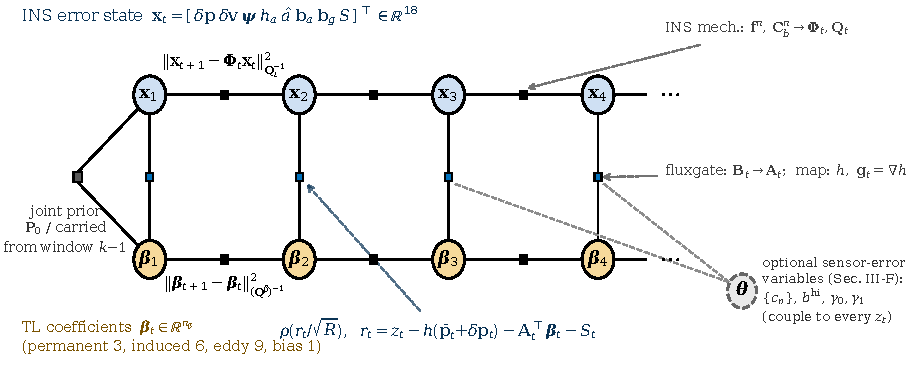
\includegraphics[width=0.96\textwidth]{figs/fig_graph.pdf}
\caption{Factor graph of one window: the 18-state INS error chain $\mathbf{x}_t$ and
the time-varying TL chain $\boldsymbol{\beta}_t$, coupled by robust
scalar-magnetometer factors. Dashed arrows are known factor parameters; the dashed
node $\boldsymbol{\theta}$ holds optional extension variables.}
\label{fig:graph}
\end{figure*}

\subsection{Fixed-lag sliding window}\label{sec:window}
A single batch over a long line with a static $\boldsymbol{\beta}$ underfits the
time-varying interference; carrying $\boldsymbol{\beta}$ as a time-varying chain over
the full line removes that limitation but at a computation and latency that grow
without bound, while a per-epoch filter, conversely, cannot use future data. We take
the middle path and process the flight in overlapping windows
of length $L_w$ with overlap $L_o$, each a batch factor graph, in the manner of
fixed-lag and incremental smoothing~\cite{kaess2012,sibley2010,leutenegger2015}.
Window $k$ spans epochs $[s_k,s_k+L_w)$; it is solved as a batch and commits only its
leading stride of $L_w-L_o$ epochs. When the window slides, the states that leave it
are marginalized out and their information is carried forward as a Gaussian prior on
the retained states of window $k{+}1$ (Fig.~\ref{fig:window}), the standard fixed-lag
marginalization of square-root SAM and sliding-window visual--inertial
estimators~\cite{dellaert2006,kaess2012,leutenegger2015,qin2018}. Because the graph is
a chain, the marginal of the departing sub-graph reduces to the forward-filtered state
at the commit boundary (a Schur complement computed for free by the forward Kalman
pass), so each overlap measurement enters the estimate exactly once. The trailing
overlap $L_o$ thus acts as bounded smoother look-ahead, giving each committed estimate
$L_o$ epochs of future data, while the marginalized handoff keeps both the mean
and the covariance consistent across window boundaries.
Algorithm~\ref{alg:window} summarizes the procedure; its per-window cost is
constant in the line length, giving overall linear complexity.

\begin{figure}[t]
\centering
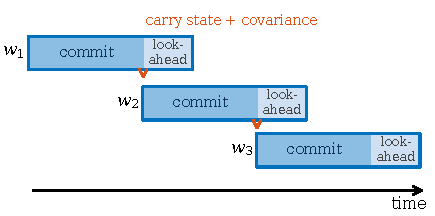
\includegraphics[width=0.98\columnwidth]{figs/fig_window.pdf}
\caption{Fixed-lag sliding window: each window commits its leading stride and
carries the smoothed state and covariance to the next; the overlap is the
look-ahead.}
\label{fig:window}
\end{figure}

\begin{algorithm}[t]
\caption{Fixed-lag sliding-window smoother}
\label{alg:window}
\begin{algorithmic}[1]
\State \textbf{Input:} measurements $\{z_t\}$, TL rows $\{\mathbf{A}_t\}$, map $h$,
window $L_w$, overlap $L_o$, prior $(\hat{\boldsymbol{\chi}}_0,\mathbf{P}_0)$
\State $s\gets 1$
\While{$s\le T$}
  \State build factor graph on epochs $[s,\min(s{+}L_w,T))$ with prior
         $(\hat{\boldsymbol{\chi}}_{s-1},\mathbf{P}_{s-1})$
  \Repeat \Comment{robust Gauss--Newton}
    \State linearize residuals \eqref{eq:resid}; form weights $w_t$ from $\rho$
           \eqref{eq:irls}
    \State solve the linearized chain by an iterated RTS pass~\cite{rauch1965}
           (equivalently, sparse QR / square-root SAM~\cite{dellaert2006};
           Sec.~\ref{sec:method}-D)
    \State update $\boldsymbol{\chi}\gets\boldsymbol{\chi}+\Delta\boldsymbol{\chi}$
  \Until{converged}
  \State commit epochs $[s,s{+}L_w{-}L_o)$; recover $(\hat{\boldsymbol{\chi}},
         \mathbf{P})$ at epoch $s{+}L_w{-}L_o{-}1$
  \State $s\gets s+(L_w-L_o)$
\EndWhile
\State \textbf{Output:} committed trajectory $\{\hat{\mathbf{p}}_t,
\hat{\boldsymbol{\beta}}_t\}$
\end{algorithmic}
\end{algorithm}

It is worth being precise about the causal failure this repairs, because the same
time-varying model~\eqref{eq:tl} can be, and is, carried inside an EKF. At cold
start the coefficient error makes the residual hundreds of nanotesla, and a
one-pass filter must apportion that residual between position and
$\boldsymbol{\beta}$ immediately, using only its current covariance, before the
maneuvers that would separate the two have occurred. A wrong apportionment moves the
position estimate, and the next update then evaluates the map gradient
$\mathbf{g}_t$ at the wrong place, so even a correct residual is charged to the
wrong direction: the linearization point and the estimate corrupt each other, and
because the filter cannot revise committed states, the loop runs open until
divergence. Innovation gating does not repair this, because the cold-start residual
is not an outlier but a systematic bias present in every early measurement:
a chi-square gate rejects essentially all of them, which removes the only evidence
from which $\boldsymbol{\beta}$ could be identified and leaves free-inertial drift.
The window changes both halves of the failure. Each Gauss--Newton iteration
relinearizes every epoch in the window, so once the coefficients begin to converge
mid-window, the residual attribution and the linearization points of the
early epochs are revised retroactively; and the robust kernel, unlike a
gate, keeps every measurement, merely down-weighting what the current model cannot
yet explain. The breadth study isolates the two effects: the window alone, with no
robust kernel, already stays bounded on every counted case, so the load-bearing mechanism is the windowed
relinearization, with the kernel as an accuracy refinement.

Two parameters govern the window: the length $L_w$ and the overlap $L_o$. $L_w$ sets
how much data each compensation estimate sees and thus the effective adaptation
time; too short and $\boldsymbol{\beta}$ is under-determined, too long and it cannot
track drift. $L_o$ sets the look-ahead and hence the commit latency: a committed
state has seen $L_o$ epochs of future data, and the estimator lags real time by
$L_o$. In the experiments we use $L_w=\SI{5}{\minute}$ and $L_o=\SI{90}{\second}$; the
window-length sweep in Fig.~\ref{fig:winlen} shows that shortening $L_w$ degrades
the long-line result, consistent with under-determination. The first window starts the
coefficients at zero under $\mathbf{P}_0^{\beta}$ and lets the FOGM disturbance state
absorb what the compensation cannot yet explain; subsequent windows inherit the
carried covariance and converge in a few Gauss--Newton iterations
(typically $3$--$5$; Sec.~\ref{sec:results}-G), which is why the per-window
iteration count stays low despite the nonlinearity of the map term. How far
$\mathbf{P}_0^{\beta}$ lets that first window travel turns out to decide whether a
short-lag smoother survives the cold start at all (Section~\ref{sec:coldprior}).

\subsection{Per-epoch incremental smoothing}\label{sec:incremental}
Taking the lag to its lower limit turns the window into a per-epoch recursion: instead
of re-solving a batch every stride, the graph is extended and re-solved once per
measurement. We realize this with an incremental fixed-lag smoother built on the
Bayes-tree factorization of iSAM2~\cite{kaess2012}. At each epoch the two chain
factors and the scalar-magnetometer factor of that epoch are added to the graph;
iSAM2 identifies the variables whose linearization the new factors disturb and
re-eliminates only that part of the Bayes tree, so the per-epoch cost does not grow
with the flight. States that leave the lag are marginalized rather than dropped: their
information is compressed into a Gaussian prior on the oldest retained state, the same
boundary marginal the sliding window carries across its handoff. The window and the
incremental smoother are therefore one estimator at two strides. The window
re-optimizes a batch every $L_w-L_o$ epochs and hands the filtered boundary forward so
each overlap measurement is counted once; the incremental smoother is the limit in
which the stride is a single epoch, with a causal estimate available at every step
from the current linearization point. Along the whole spectrum the lag alone sets how
much future data corrects a committed state, hence its accuracy, latency, and
per-epoch cost together.

One numerical point matters for reproduction. The position channel of the discrete
process covariance $\mathbf{Q}_t$ is minute, of order $10^{-31}\,\mathrm{rad}^2$ in
the horizontal-position states, because position error is driven only through velocity
over a single sample; whitening the process factor by $\mathbf{Q}_t^{-1/2}$ then spans
some thirty orders of magnitude. A Cholesky factorization of the information matrix
squares this conditioning and fails outright, returning an indeterminate variable. Two
changes remove the failure: a floor of $10^{-20}\mathbf{I}$ added to $\mathbf{Q}_t$,
which injects under a millimetre of position uncertainty per step and is dynamically
negligible, and a QR factorization of the square-root information matrix in place of
Cholesky, which operates on the square root and so tolerates the residual spread. A
larger floor or per-epoch regularizing priors also suppress the exception, but by
pinning the estimate onto the propagated INS they defeat the correction; the
floor-plus-QR combination keeps the estimate free while remaining numerically stable,
and is what both the incremental and the batch solvers use.

\subsection{Robust kernel and sparse solver}
Map error and transient interference produce heavy-tailed
residuals that a quadratic cost over-weights. We use a Huber kernel~\cite{huber1964}
\begin{equation}
\rho(u)=\begin{cases}\tfrac12 u^2,& |u|\le\delta,\\
\delta\big(|u|-\tfrac12\delta\big),& |u|>\delta,\end{cases}
\label{eq:huber}
\end{equation}
minimized by iteratively reweighted least squares (IRLS): each Gauss--Newton
iteration reweights measurement factor $t$ by
\begin{equation}
w_t=\min\!\big(1,\;\delta/|u_t|\big),\qquad u_t=r_t/\sqrt{R},
\label{eq:irls}
\end{equation}
so gross outliers are down-weighted toward an absolute-value penalty while inliers
keep the efficient quadratic cost. In the implementation the reweighting is applied
from the second Gauss--Newton iteration onward (the first iteration is plain least
squares) with $w_t$ clamped to $[10^{-6},1]$, and $\delta=1.345$ gives the standard
$95\%$ Gaussian efficiency. Alternatives such as switchable
constraints~\cite{sunderhauf2012} and dynamic covariance
scaling~\cite{agarwal2013} fit the same graph interface and could replace
\eqref{eq:huber} unchanged.

Each Gauss--Newton iteration solves a sparse linear system whose Jacobian has the
block-bidiagonal structure of the two chains in Fig.~\ref{fig:graph} (in the
static-$\boldsymbol{\beta}$ limit the coefficient blocks collapse to one shared
column). We factor it
by column-pivoted QR on the square-root information matrix (square-root
SAM~\cite{dellaert2006,dellaert2017}), which is numerically stable and exploits the
chain sparsity. In the Gaussian case an iterated RTS pass~\cite{rauch1965} returns
the identical estimate:

\begin{lemma}\label{lem:rts}
Under Assumption~\ref{as:model}, with $\rho(u)=\tfrac12u^2$ and $\boldsymbol{\beta}$
held fixed, the minimizer of~\eqref{eq:cost} equals the Rauch--Tung--Striebel (RTS)
smoother estimate over the window.
\end{lemma}
\begin{IEEEproof}
With $\rho$ quadratic and $\boldsymbol{\beta}$ fixed, \eqref{eq:cost} is the
negative log-density of a linear--Gaussian chain, so its minimizer is the posterior
mean, which the forward Kalman and backward RTS passes
compute~\cite{rauch1965}.
\end{IEEEproof}

The lemma serves two ends. It licenses the fast iterated-RTS solve on the
navigation chain, which we check against the QR path to within a metre in
Section~\ref{sec:results}-A; and it fixes scope, since the paper's gain comes from
precisely what the lemma's hypotheses exclude: the jointly estimated, time-varying
$\boldsymbol{\beta}$, the robust kernel~\eqref{eq:huber}, and the fixed-lag window.

\section{Separability of Position and Compensation}
\label{sec:observability}
Whether position can be recovered while the compensation is estimated jointly is a
property of the measurement geometry. Over a window let $\mathbf{G}$ have rows
$\mathbf{g}_t^{\!\top}$ (the map-gradient/position sensitivity) and let
$\boldsymbol{\Psi}$ have rows $\mathbf{A}_t^{\!\top}$ (the TL regressor). To
isolate the position--compensation coupling, restrict~\eqref{eq:meas} to the
$(\delta\mathbf{p},\delta\boldsymbol{\beta})$ subspace, giving the window model
$\mathbf{z}=\mathbf{G}\,\delta\mathbf{p}+\boldsymbol{\Psi}\,\delta\boldsymbol{\beta}+\boldsymbol{\eta}$
(Fig.~\ref{fig:obs}). This model freezes $\delta\mathbf{p}$ and
$\delta\boldsymbol{\beta}$ over the window: it is a per-window surrogate for the
time-varying system~\eqref{eq:dyn},~\eqref{eq:resid} that isolates the
position--compensation coupling. It holds the coefficients fixed and sets aside the
slow magnetic-bias state $S_t$ and the INS dynamics that a full observability Gramian
would mix in, so it speaks to how position and compensation are told apart, not to
observability of the complete time-varying state.

\begin{figure}[t]
\centering
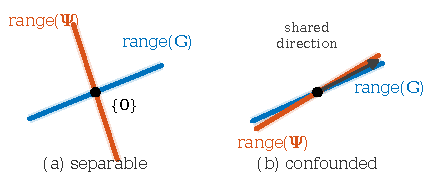
\includegraphics[width=0.98\columnwidth]{figs/fig_obs.pdf}
\caption{Observability geometry (Proposition~\ref{prop:obs}): position and
compensation are separable when range$(\mathbf{G})$ and range$(\boldsymbol{\Psi})$
meet only at the origin (left) and confounded when they share a direction (right).}
\label{fig:obs}
\end{figure}

\begin{proposition}\label{prop:obs}
A position perturbation $\delta\mathbf{p}$ is indistinguishable from a
compensation adjustment, hence unobservable from map matching over the
window, if and only if $\mathbf{G}\,\delta\mathbf{p}\in\mathrm{range}(\boldsymbol{\Psi})$.
Consequently the joint state $(\delta\mathbf{p},\delta\boldsymbol{\beta})$ is
observable if and only if the stacked matrix
$[\,\mathbf{G}\;\;\boldsymbol{\Psi}\,]$ has full column rank; equivalently, if and
only if all three of the following hold:
(i) $\ker\mathbf{G}=\{\mathbf{0}\}$ (the map gradient excites every
position direction over the window);
(ii) $\ker\boldsymbol{\Psi}=\{\mathbf{0}\}$ (the compensation basis has
full column rank); and
(iii)
$\mathrm{range}(\mathbf{G})\cap\mathrm{range}(\boldsymbol{\Psi})=\{\mathbf{0}\}$
(no shared direction). Condition (iii) alone governs the
position--compensation confounding: when it fails, a position shift with
$\mathbf{G}\,\delta\mathbf{p}\neq\mathbf{0}$ is reproduced exactly by a
compensation change.
\end{proposition}

\begin{IEEEproof}[Proof sketch]
Two joint states are indistinguishable exactly when their difference lies in
$\ker[\,\mathbf{G}\;\;\boldsymbol{\Psi}\,]$, so observability is full column
rank of the stacked matrix; sorting the kernel elements by whether
$\mathbf{G}\,\delta\mathbf{p}$ vanishes yields conditions (i)--(iii). The full
proof is in Appendix~\ref{app:proof}.
\end{IEEEproof}

Condition (iii) is the operative one in practice. Conditions (i) and (ii) are
routine to check; the confounding of position with compensation, by contrast,
depends on the joint geometry of the flight path and the local map gradient, and it
can fail only through coincidence of the flown attitude history with that
gradient, plausible, for instance, when turns always occur at the same map features.
One expects (iii) to hold for trajectories and maps in general position, but the
condition is non-constructive: it yields no reliable scalar screening statistic, and
in our experiments correlation-based proxies for the intersection (in-sample basis
$R^2$, out-of-sample prediction, gradient-alignment indices) did not generalize
across estimators or lines. We report that as a negative result, not a predictive
test.

\begin{remark}\label{rem:gauge}
Condition (ii) fails, or very nearly fails, for the classical TL basis itself: with
unit direction cosines the three induced diagonal columns sum to
$B_t(u^2{+}v^2{+}w^2)=B_t$, which is collinear with the constant-bias column to the
degree that the total field is constant over a window ($B_t$ varies by well under a
percent of its \SI{5e4}{\nano\tesla} magnitude), the long-known collinearity of TL
regression~\cite{leliak1961,noriega2015}. This is, to that approximation, a gauge
freedom of the compensation rather than a navigation defect: a perturbation
$\delta\boldsymbol{\beta}$ in the near-null subspace of $\boldsymbol{\Psi}$ moves
the predicted interference $c_t=\mathbf{A}_t^{\top}\boldsymbol{\beta}_t$, and hence
the position estimate, only negligibly. The prior $\mathbf{P}_0$ and the
random-walk factors select one representative of each near-gauge orbit.
Separability of position from compensation is governed by (iii) alone and is
unaffected.
\end{remark}

\begin{remark}\label{rem:floor}
The condition is geometric: it depends on the ranges of $\mathbf{G}$ and
$\boldsymbol{\Psi}$ over the window, hence on the flight path and the local map
gradient. It explains the dominant failure mode seen in practice: over a locally
flat map $\mathbf{G}\!\approx\!\mathbf{0}$ and condition (i) fails, so position is
unobservable regardless of the compensation, a map-information floor that bounds
every estimator, which we observe on the shortest line in Section~\ref{sec:results}.
\end{remark}

The cold-start transient observed in real time makes this confounding visible. A
per-epoch smoother with a short lag (Section~\ref{sec:incremental}), run from a cold
start on line 1007.06 Mag~5, holds a horizontal DRMS near \SI{82}{\meter} through the
first several minutes before locking on (Fig.~\ref{fig:warmstart}). Seeding the
compensation with a warm Tolles--Lawson prior, tightening its initial standard
deviation from \num{1.0} to \num{0.1}, removes only about \SI{40}{\percent} of this transient, to
roughly \SI{50}{\meter}; the remainder is not a compensation error but a
map-observability one, precisely conditions~(i) and~(iii) of
Proposition~\ref{prop:obs} early in the flight. Two observations separate the causes.
First, the same cold start with a long lag shows no transient at all: given enough
future gradient, the smoother resolves the position--compensation ambiguity that the
short lag cannot. Second, the cold and warm runs lock on at the same instant, when the
aircraft crosses a strong map feature about four and a half minutes in, rather than
after a fixed compensation-learning time. Both point to the map gradient, not the
compensation prior, as what ultimately breaks the confounding: where
$\mathrm{range}(\mathbf{G})$ is rich the two unknowns separate, and a warm prior only
shortens the wait; Fig.~\ref{fig:warmstart} shows the decomposition on the first six
minutes of the segment.

That decomposition holds for a magnetometer whose uncompensated field the
compensation prior can represent. It does not hold for the cabin magnetometer with
the larger platform field, where the prior itself is the binding constraint and
neither a longer lag nor a richer map gradient recovers the estimate;
Section~\ref{sec:coldprior} separates that case and reports the settings under which
it is bounded. The two statements are about different regimes and we keep them
apart: in the first regime the compensation can reach the interference and is merely
slow; in the second it cannot reach it at all.

\begin{figure}[t]
\centering
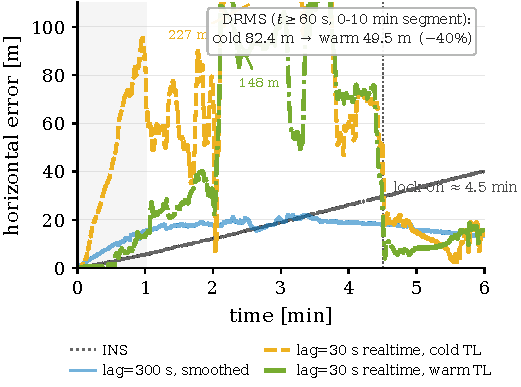
\includegraphics[width=\columnwidth]{figs/fig_warmstart.pdf}
\caption{First six minutes of the cold-start transient at a \SI{30}{\second} lag: a
warm compensation prior cuts the penalty by \SI{40}{\percent}, but both runs lock on only at
the strong map feature near four and a half minutes.}
\label{fig:warmstart}
\end{figure}

\section{Experiments and Results}\label{sec:results}

\subsection{Dataset, maps, and protocol}
All experiments use the public SGL~2020 challenge dataset~\cite{gnadt2020}: a
Cessna~208B instrumented with a flight-grade INS, several onboard scalar
magnetometers (a compensated tail-stinger sensor and uncompensated cabin sensors
Mag~4 and Mag~5, all optically-pumped cesium-vapor units), a three-axis fluxgate,
and reference truth. The flights serve distinct purposes, and we choose lines
accordingly. Flt1007 is the free-flight mission, in which the aircraft flies freely
within the mapped Renfrew ($\approx\!\SI{400}{\meter}$) and Eastern/Perth
($\approx\!\SI{800}{\meter}$) areas, so its lines are the closest to a navigation
task and are what prior work~\cite{gnadt2020,canciani2017,hager2026} reports;
1007.06 is our primary line for that reason. Flt1003 is a crustal-field
measurement flight (survey traverses at \num{400} and \SI{800}{\meter});
its lines 1003.02 and 1003.08 are straighter than the free-flight legs. Flt1006 is
a calibration-maneuver flight, so we set its single short line aside, and the map-building flights (Flt1004--1005) are not
used. Two honest points remain. First, none of these is a dedicated long,
straight-and-level operational transit; the free-flight and survey legs carry more
attitude variation, which stresses compensation but also aids TL
observability by exciting the regressor, so
performance on a pure operational cruise is not directly established here and is
future work. Second, the lines span two altitude regimes: four at the
$\approx\!\SI{400}{\meter}$ survey-drape altitude and 1007.02 at
$\approx\!\SI{800}{\meter}$, where upward continuation attenuates the anomaly.
Map matching uses the Eastern (``E'') and Renfrew (``R'') high-resolution anomaly
grids, upward-continued to flight altitude with the IGRF core field restored. The
metric is horizontal distance-RMS (DRMS) of position error after a
\SI{10}{\minute} warm-up. Cold
start means the TL coefficients are initialized to zero with no calibration flight;
the navigation solution is accurately initialized (position std \SI{0.1}{\meter},
Table~\ref{tab:params}), so the term denotes a compensation cold start, not an
unknown-position navigation start.
For every comparison the EKF and FGO estimators use identical dynamics, map
interpolation, and noise settings (Table~\ref{tab:params}); the window smoother
additionally applies the Huber kernel~\eqref{eq:huber}, whose isolated
contribution is reported separately in Table~\ref{tab:1007}
(\num{33.0}$\rightarrow$\SI{30.7}{\meter} on Mag~4), so the reader can attribute
the remaining margin to the estimator structure. Unless noted, the window smoother
uses $L_w=\SI{5}{\minute}$ and $L_o=\SI{90}{\second}$; $L_w$ was selected on line
1007.06 (Fig.~\ref{fig:winlen}) and then held fixed for every other line, so the
breadth results of Table~\ref{tab:breadth} are not per-line tuned. All numbers are
produced by scripted runs under a fixed software environment and are available from
the authors on request.

\begin{table}[t]
\caption{Estimator settings for all cold-start results; the same $\mathbf{P}_0$,
$\mathbf{Q}$, $R$, and TL settings drive both the EKF and the smoother.}
\label{tab:params}
\centering
\footnotesize
\setlength{\tabcolsep}{3pt}
\begin{tabular}{@{}llr@{}}
\toprule
Group & Parameter & Value \\
\midrule
Measurement & noise std.\ $\sqrt{R}$ & \SI{12}{\nano\tesla} \\
FOGM $S$ & $(\sigma_S,\tau)$ & \SI{3}{\nano\tesla}, \SI{180}{\second} \\
Initial $\mathbf{P}_0$ & pos.\ / alt.\ std. & \num{0.1} / \SI{1.0}{\meter} \\
 & velocity std.\ (per axis) & \SI{1.0}{\meter\per\second} \\
TL prior / walk & $\mathbf{P}_0^{\beta}$;\; $\mathbf{Q}^{\beta}$ &
  $\mathbf{I}(\sigma_{\beta})^2$;\; $\mathbf{I}(1.0)^2\Delta t$ \\
 & $\sigma_{\beta}$ (window, batch, Sec.~\ref{sec:observability}) & 1.0 \\
 & $\sigma_{\beta}$ (per-epoch, Sec.~\ref{sec:coldprior}) & 100 \\
TL basis & terms (App.~\ref{app:tl}) & P{+}I{+}E{+}bias (19) \\
Window & $L_w$ / $L_o$ / $\Delta t$ [s] & 300 / 90 / 0.1 \\
Robust & Huber $\delta$ & 1.345 \\
 & IRLS & 2nd iter.\ on, $w\in[10^{-6},1]$ \\
Gauss--Newton & max.\ iter.\ / tol. & 5 / $10^{-4}$ \\
\bottomrule
\end{tabular}
\end{table}

For geographic context, Fig.~\ref{fig:map} shows line 1003.02 over the Eastern
anomaly field. As a controlled check on the compensated stinger, before the
cold-start problem, the batch factor graph tightens the horizontal DRMS from the
EKF's \SI{31.5}{\meter} to \SI{14.0}{\meter}, against \SI{114.4}{\meter}
free-inertial (Fig.~\ref{fig:poserr}); its iterated-RTS and sparse-GN/QR solvers
agree to within \SI{1}{\meter}, an empirical check of Lemma~\ref{lem:rts}.

\begin{figure}[t]
\centering
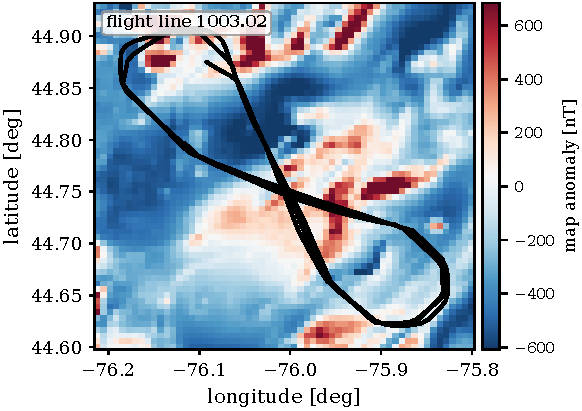
\includegraphics[width=0.98\columnwidth]{figs/fig_map.pdf}
\caption{Line 1003.02 over the Eastern anomaly map.}
\label{fig:map}
\end{figure}

\begin{figure}[t]
\centering
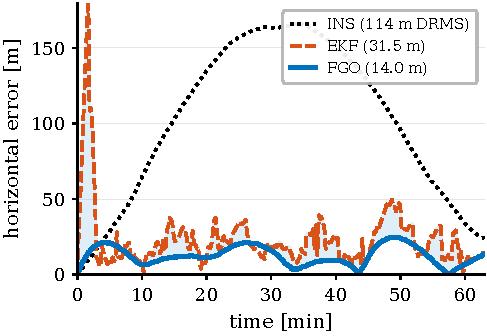
\includegraphics[width=0.98\columnwidth]{figs/fig_poserr.pdf}
\caption{Horizontal position error on line 1003.02: batch FGO, EKF, and free
inertial (DRMS in the legend).}
\label{fig:poserr}
\end{figure}

\subsection{Baselines}\label{sec:baseline}
The strong causal competitor is the online EKF+TL+NN lineage that augments the
Pinson error state with the TL coefficients $\boldsymbol{\beta}$ and the weights of
a small feed-forward network, all propagated as filter states and updated
online~\cite{gnadt2022,hager2026}. We run its reference
implementation~\cite{gnadt2022}, tuned by us for a stable cold start, and do not
claim to reproduce the extended filter of~\cite{hager2026}. Cold start forces one
substantive change: with no calibration flight to warm-start from, we initialize the
network output normalization data-drivenly from the first five minutes of onboard
interference; a naive port instead drives the network bias to
$\sim\!5\times10^{4}$\,nT and the filter to \texttt{NaN}. We keep the uncompensated
scalar out of the network inputs, as Proposition~\ref{prop:obs}(iii) requires: a
position-dependent input carries sensitivity $\mathbf{g}_t$, so the network absorbs
the map signal and position drifts while the residual stays small (the
scalar-augmented variant~\cite{hager2026} escapes this only by freezing the network
after its transient). The tuned filter uses the permanent TL group with an
eight-unit hidden layer, a FOGM $(\sigma,\tau)=(\SI{3}{\nano\tesla},\SI{180}{\second})$,
and measurement variance $12^2\,\mathrm{nT}^2$, reaching \num{48.8}/\SI{18.3}{\meter}
on Mag~4/5 (Table~\ref{tab:1007}), consistent with published cold-start operating
points~\cite{gnadt2022,hager2026}. We also compare a weak online-TL EKF and a
marginalized particle filter carrying the TL coefficients; all are our own runs under
one protocol, except the particle filter, reported under its most favorable per-case
configuration.

\subsection{Cold-start line vs.\ online EKF+TL+NN}
The central comparison is the cold start on uncompensated cabin magnetometers,
where the interference is present and must be learned online. Table~\ref{tab:1007}
and Fig.~\ref{fig:coldstart} report the primary evaluation line 1007.06
(\SI{87}{\minute}, full length) on Mag~4 and Mag~5. A static-TL batch forces a
single coefficient vector over the whole line; it underfits the time-varying
interference and degrades to \num{123.7}/\SI{68.1}{\meter}. Allowing the
compensation to adapt with a \SI{5}{\minute} window recovers it to
\num{33.0}/\SI{13.5}{\meter}, and the Huber kernel further trims transient outliers
to \num{30.7}/\SI{13.1}{\meter}. Taking the lag to its per-epoch limit, with the
compensation prior of Section~\ref{sec:coldprior}, gives
\num{24.2}/\SI{11.5}{\meter} committed at a \SI{300}{\second} lag and
\num{42.7}/\SI{16.0}{\meter} causally, with no look-ahead at all. Our online
EKF+TL+NN baseline reaches \num{48.8}/\SI{18.3}{\meter}. The per-epoch smoother
beats the NN-augmented filter on both sensors, \SI{24.6}{\meter} on Mag~4 and
\SI{6.8}{\meter} on Mag~5, without any neural network, using only the linear TL
basis carried as graph variables; the comparison holds even when the smoother is
read causally, where it is ahead by \SI{6.1}{} and \SI{2.3}{\meter}. All compared numbers are our own runs under one
protocol; 1007.06 is the line on which the baseline tuning is anchored, and the
same baseline carries to the other lines in the breadth study
(Table~\ref{tab:breadth}). We attribute the
margin to the window look-ahead: the coefficients are identified from data on both
sides of each committed epoch, whereas the EKF must commit with past data only.

The window length itself trades under-determination against staleness.
Fig.~\ref{fig:winlen} plots DRMS across window lengths on this line: the full-line
static batch cannot track the coefficient drift, windows that are too short
under-determine them, and the \SI{5}{\minute} window and longer stay bounded, with
\SI{5}{\minute} balancing adaptation against under-determination. The tradeoff
mirrors the expressiveness discussion of
Section~\ref{sec:observability} and makes $L_w$ a physically interpretable knob
rather than a free hyperparameter; a denser sweep across more lines, where the
balance can shift toward longer windows, is left to future work.

\begin{figure}[t]
\centering
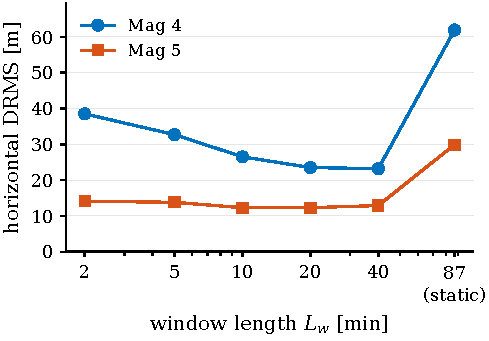
\includegraphics[width=0.92\columnwidth]{figs/fig_winlen.pdf}
\caption{Window length $L_w$ versus horizontal DRMS on line 1007.06 (cold start).}
\label{fig:winlen}
\end{figure}

\begin{table}[t]
\caption{Cold start on line 1007.06 (Flt1007), uncompensated cabin magnetometers;
DRMS [m]. INS \SI{318}{\meter}; compensated-Mag~1 EKF $\approx\SI{20}{\meter}$.}
\label{tab:1007}
\centering
\begin{tabular}{lrr}
\toprule
Method (no NN unless noted) & Mag 4 & Mag 5 \\
\midrule
FGO-online, static batch TL & 123.7 & 68.1 \\
FGO-online, window \SI{5}{\minute} & 33.0 & 13.5 \\
FGO-online, window \SI{5}{\minute} + Huber & 30.7 & 13.1 \\
\textbf{FGO-online, per-epoch, \SI{300}{\second} lag} & \textbf{24.2} & \textbf{11.5} \\
\quad same, causal (zero look-ahead) & 42.7 & 16.0 \\
\midrule
EKF+TL+NN, online~\cite{gnadt2022,hager2026} & 48.8 & 18.3 \\
\bottomrule
\end{tabular}
\end{table}

\begin{figure}[t]
\centering
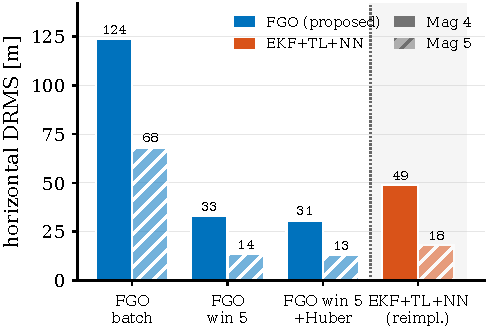
\includegraphics[width=0.98\columnwidth]{figs/fig_coldstart.pdf}
\caption{Cold start on line 1007.06: the NN-free factor graph across the lag
spectrum (left, per-epoch smoother highlighted) versus the online EKF+TL+NN
baseline (right).}
\label{fig:coldstart}
\end{figure}

These cold-start numbers also settle a question the formulation raises: with no
neural network, how does the estimator cope with the large fraction of the cabin
interference that the linear TL basis cannot span. The mechanism is the one built in
Section~\ref{sec:method}-A, where the time-varying coefficients, the FOGM
disturbance state, and the robust kernel together absorb that remainder as a
structured robust regression. The trade it makes is visible in the numbers. The
network buys a lower compensation residual, while the window, the disturbance state,
and the robust kernel together buy navigation robustness at a higher residual. This
is why the uncompensated Mag~4 DRMS of tens to hundreds of metres sits well above
survey-grade compensation and still bounds the inertial drift. A learned residual
could be added later as an extra factor on the same measurement, for example a
Gaussian-process or small-network term, which would place the network's
expressiveness inside the graph rather than inside a filter; we leave that to future
work.

\subsection{Breadth across lines, flights, and maps}
Table~\ref{tab:breadth} runs the same cold-start TL model on four long lines
spanning two flights and two maps, free-flight navigation legs (Flt1007) and
survey traverses (Flt1003), grouped by purpose, against two
linearized baselines: the plain online-TL EKF and the online EKF+TL+NN of
Section~\ref{sec:baseline} (the strong causal method that a fair comparison
demands). A marginalized (Rao-Blackwellized) particle filter carrying the TL
coefficients in its conditionally-linear-Gaussian block (MPF+TL), a genuine
non-Gaussian Bayesian estimator rather than a linearization, is examined
separately below.

The baselines behave very differently, and the contrast is the point. The
plain online-TL EKF is fragile: on the noisy Mag~4 it diverges from the cold start
to tens of kilometres on two lines and runs off the map on a third. The neural
network is what fixes this: the EKF+TL+NN stays finite on all eight cases,
confirming that its residual network is what buys cold-start robustness for the
causal filter. The per-epoch smoother matches that robustness without any neural
network (it is bounded on all eight) and improves on accuracy: across the four
full-length lines (\SIrange{63}{87}{\minute}, eight mag-cases) it is the best of
the four estimators on all eight, beating the NN-augmented filter by
\SIrange{6.8}{101.6}{\meter} (Fig.~\ref{fig:breadth}); read causally, with no
look-ahead at all, it is still ahead on six of the eight, the exceptions being
1007.02 Mag~5 (\num{33.1} against \SI{30.4}{\meter}) and 1003.08 Mag~4
(\num{48.9} against \SI{46.6}{\meter}); the particle filter, reported
separately, diverges on these cases.

The marginalized particle filter is reported separately because it resists a
single-number summary. Implemented as the reference RBPF (bootstrap proposal,
systematic resampling, and the same conditionally-linear TL block) and given its
most favorable per-case configuration, with the measurement noise matched to the
residual, resampling at half the effective sample size, and regularization
roughening, it is erratic at cold start: bounded near \SI{40}{\meter} only on the
cleanest Mag~5 legs, degrading to hundreds of metres or kilometres, with a strong
run-to-run (seed) dependence, elsewhere. With the toolbox default settings it
diverges outright. On no counted case does it come within a factor of two of the
window, and its position covariance is severely over-confident (the consistency
study below). The sensitivity is itself the finding: a sequential particle
representation needs the case-by-case tuning to stay bounded at cold start that the
batch window does not, so a non-Gaussian representation alone does not substitute
for the re-smoothing.

We also ran the short calibration-maneuver line 1006.08 (Flt1006) but set it aside
rather than tabulate it: it is only \SI{14}{\minute} long, so the \SI{10}{\minute}
warm-up leaves a \SI{4}{\minute} window over which none of the DRMS values is
reliable, and its low map-information floor (the Remark in
Section~\ref{sec:observability}) makes every method weak. It reproduces the same causal-EKF divergence, but we draw no
accuracy conclusion from it: in particular the NN's \SI{108.3}{\meter} on its Mag~5,
against \SIrange{117}{122}{\meter} for the TL-only EKF and window, is not evidence of
an NN accuracy advantage on a window this short.

Two effects in the reliable cases are worth naming. First, the EKF+TL+NN follows
the reproduced design in feeding the network only the permanent TL group,
whereas the online-TL EKF and the window smoother both carry the full
permanent-induced-eddy-bias basis; on the well-conditioned Mag~5 those linear
higher-order terms matter, so the NN filter can fall behind even the plain
EKF (1003.02: $29.5$ vs \SI{28.1}{\meter}) when its network has not yet learned
what the dropped linear terms would have supplied directly. Second, and relatedly,
the network's extra online-learned states add estimation variance where the linear
basis already suffices, a cost the NN-free window avoids. Both effects favor a
linear compensation carried in a smoother over a learned one carried in a filter,
on this benchmark. One caveat on provenance: the EKF+TL+NN is the lineage's
reference implementation under our tuning, matching the reported 1007.06 operating
points to within a few metres, but the original's per-line numbers on the other
lines are unpublished, so the comparison is against a faithful, not the
authors', filter. Its cold-start trajectory is also numerically sensitive, so its
per-line DRMS varies between runs; the values here are those of a single fixed run
and do not affect the best-of-three ordering.

\begin{table}[t]
\caption{Breadth: cold-start cabin magnetometers, DRMS [m]. Purpose FF = free-flight
(Flt1007), SV = survey (Flt1003); ``div.''\ $>\SI{10}{\kilo\meter}$, ``err.''\ = off
map. The proposed estimator is the per-epoch smoother of
Section~\ref{sec:incremental} at $\sigma_{\beta}=100$, reported twice: its causal
output, which is the like-for-like comparison against the two causal filters, and
its committed output at a \SI{300}{\second} lag. The sliding window is kept as the
intermediate point of the lag spectrum, at its own \SI{90}{\second} commit
latency. Bold marks the best causal estimator and the best overall. The
marginalized particle filter (MPF+TL) is treated separately in the text: even at
its most favorable per-case tuning it is erratic and never competitive.
Calibration line 1006.08 set aside (see text).}
\label{tab:breadth}
\centering
\setlength{\tabcolsep}{3pt}
\begin{tabular}{llccc rr rr r}
\toprule
 & & & alt & & EKF & EKF+ & \multicolumn{2}{c}{FGO per-epoch} & FGO \\
\cmidrule(lr){8-9}
Line & Purp. & Map & [km] & Mag & online & TL+NN & causal & \SI{300}{\second} & win \\
\midrule
1007.06 & FF & R & 0.4 & 4 & 46.7 & 48.8 & \textbf{42.7} & \textbf{24.2} & 30.7 \\
1007.06 & FF & R & 0.4 & 5 & 17.8 & 18.3 & \textbf{16.0} & \textbf{11.5} & 13.1 \\
1007.02 & FF & E & 0.8 & 4 & div. & 130.0 & \textbf{74.3} & \textbf{28.4} & 39.9 \\
1007.02 & FF & E & 0.8 & 5 & 31.6 & 30.4 & 33.1 & \textbf{15.8} & 15.4 \\
1003.02 & SV & E & 0.4 & 4 & div. & 101.0 & \textbf{58.2} & \textbf{19.6} & 43.1 \\
1003.02 & SV & E & 0.4 & 5 & 28.1 & 29.5 & \textbf{21.9} & \textbf{12.0} & 21.1 \\
1003.08 & SV & R & 0.4 & 4 & err. & \textbf{46.6} & 48.9 & \textbf{25.0} & 28.0 \\
1003.08 & SV & R & 0.4 & 5 & 21.1 & 20.7 & \textbf{19.2} & \textbf{10.5} & 13.1 \\
\midrule
\multicolumn{5}{l}{best of the causal estimators} & & & \textbf{6 / 8} & & \\
\multicolumn{5}{l}{best overall} & & & & \textbf{8 / 8} & \\
\bottomrule
\end{tabular}
\end{table}

\begin{figure}[t]
\centering
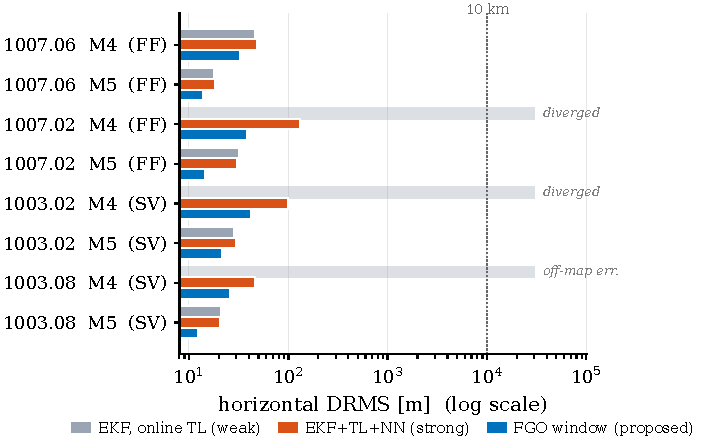
\includegraphics[width=0.92\columnwidth]{figs/fig_breadth.pdf}
\caption{Breadth study (Table~\ref{tab:breadth}), log DRMS axis: online-TL EKF
(gray), EKF+TL+NN (red), and the NN-free per-epoch FGO at a \SI{300}{\second} lag
(blue). The sliding window is the intermediate lag and is tabulated rather than
plotted; the MPF+TL particle filter is erratic at cold start (see text) and is
omitted.}
\label{fig:breadth}
\end{figure}

Two conclusions follow, and they are worth separating because a single-line
comparison conflates them. The first is about robustness. Keeping a causal filter
bounded at cold start is not unique to the window, since the neural network does it
too, so the blanket claim that causal filters diverge is false for the
state-of-the-art filter. It is, however, true of every non-NN cold-start estimator
we tried: the plain online-TL EKF diverges, and the marginalized particle filter,
though a full Bayesian estimator, is only erratically bounded and never competitive
(preceding paragraph). Reliable cold-start compensation without a network requires
the batch/window re-smoothing, not merely a non-Gaussian representation. An ablation within our own estimator locates the
mechanism more precisely: running the same window with the robust kernel disabled
still stays bounded on all eight counted cases (e.g.\ \SI{60.3}{\meter} on
1003.02/Mag~4 where the causal filter reads \SI{41626}{\meter}, refined to
\SI{43.1}{\meter} by Huber), so the robustness comes from the windowed
relinearization of Section~\ref{sec:method}-B, and the kernel buys accuracy, not
survival. The recorded platform currents let us check the absorption account of
Section~\ref{sec:method}-A directly on line 1003.02: the fourteen onboard current
channels linearly explain \SIrange{28}{39}{\percent} of the raw cabin interference
(strobe lights, cabin fuel pump, and INS heater lead), but only
\SIrange{2}{6}{\percent} of the post-fit windowed-FGO residual, so the
current-aligned component is almost entirely absorbed by the time-varying
$\boldsymbol{\beta}_t$ and $S_t$; and the Huber-down-weighted epochs concentrate
$2.6$--$3.6\times$ on current-switching activity, with strobe switching alone
correlating at $0.55$ with the residual magnitude on Mag~5, confirming that the
kernel attenuates precisely the transients the linear states cannot track. These
are instantaneous linear regressions, hence lower bounds on the current
contribution. What the factor graph adds is that it reaches the same bounded
regime without the network, its online-training machinery, or the verification
burden that comes with it. The second is about accuracy, where the per-epoch
smoother is the best of the four on all eight full-length cases; under a paired sign test on the
per-case DRMS the one-sided probability of this count arising by chance is
$2^{-8}\approx0.004$. This margin is real, but it should
be read with care, because our EKF+TL+NN is a tuned reference implementation and part of its
deficit is that its online-learned states add variance on the well-conditioned
sensor, where the linear TL basis already suffices. The defensible reading is that a
linear estimator with no network, given future context through the window, is enough
both to survive the cold start and to match or beat an NN-augmented causal filter on
this benchmark. Table~\ref{tab:compare} places the estimator families along the axes
that matter for cold-start compensation.

The separability condition of Section~\ref{sec:observability} accounts for the
pattern. The map-information floor
(Remark~\ref{rem:floor}) is why the short calibration line 1006.08 is hard for every method, since
there is little independent map gradient to exploit over its brief window, and it is
the reason we set that line aside. The condition is geometric and predictive only
through these qualitative rules; a scalar screening statistic we tried did not
generalize, which we report as a negative result.

\begin{table}[t]
\caption{Estimator families for cold-start map-matching compensation.
\ding{51}\,= yes, \ding{55}\,= no, ($\sim$)\,= limited.}
\label{tab:compare}
\centering
\setlength{\tabcolsep}{3.5pt}
\begin{tabular}{lcccc}
\toprule
 & Future & Comp. & Robust & Bounded \\
Estimator & data & state & meas. & latency \\
\midrule
Causal EKF~\cite{canciani2017} & \ding{55} & ($\sim$) & \ding{55} & \ding{51} \\
Particle / grid filter~\cite{nordlund2009} & \ding{55} & \ding{55} & \ding{51} & \ding{51} \\
Online EKF+TL+NN~\cite{gnadt2022,hager2026} & \ding{55} & \ding{51} & ($\sim$) & \ding{51} \\
Batch FGO & \ding{51} & \ding{51} & \ding{51} & \ding{55} \\
Proposed (fixed-lag FGO) & \ding{51} & \ding{51} & \ding{51} & \ding{51} \\
\bottomrule
\end{tabular}
\end{table}

\subsection{Consistency and statistical significance}
Each real line provides a single physical realization, so its DRMS is a point
estimate and its measurement noise cannot be resampled. To assess statistical
significance and, more importantly, whether the reported covariance is credible, we
run a Monte-Carlo study in simulation, where repeated realizations are valid. We fix
one simulated trajectory over the high-resolution Eastern anomaly map and, for each
of \num{30} seeds, draw an independent INS-error realization and an independent clean
scalar-measurement realization, then run three map-matching estimators on the same
draw: the causal EKF, the marginalized (Rao-Blackwellized) particle filter already
in the toolbox, and the batch factor graph. The clean compensated measurement
isolates the navigation covariance from the cold-start compensation transient.

Averaged over the \num{30} seeds, after a \SI{30}{\second} warm-up, the horizontal
DRMS is \SI{1.4}{\meter} for the factor graph, \SI{4.1}{\meter} for the EKF, and
\SI{4.9}{\meter} for the particle filter, with \SI{95}{\percent} confidence
half-widths of \num{0.2}, \num{0.4}, and \SI{0.8}{\meter}. Even on this clean
sensor the factor graph separates cleanly from both recursive baselines (its
interval does not overlap theirs), while the EKF and the particle filter are
statistically indistinguishable in accuracy. The larger cold-start separations are
in Sections~\ref{sec:results}-C and~\ref{sec:results}-D; the purpose of this study
is consistency.

For consistency we use the per-axis two-degree-of-freedom position NEES,
$(e_N/\sigma_N)^2+(e_E/\sigma_E)^2$, whose expectation under a consistent covariance
is \num{2}. Averaged over all seeds and epochs the ANEES is \num{1.57} for the
factor graph and \num{1.72} for the EKF, both below the ideal \num{2}: both report
conservative uncertainty that bounds the true error with margin. The toolbox
particle filter is the opposite: its ANEES is \num{59.8}, more than an order of
magnitude above \num{2}, the particle-depletion signature in which the surviving
particles after resampling on a high-resolution map cluster far more tightly than the
true error and the empirical covariance collapses. This over-confidence is a
configuration artifact, not a property of the estimator class: adding regularization
roughening restores consistency (ANEES \num{1.8} at \SI{1}{\meter} roughening) at a
small accuracy cost. Even so, the factor graph dominates both recursive baselines, more
accurate (\num{1.4} versus \SIrange{4.1}{4.6}{\meter}) and consistent at once.
Fig.~\ref{fig:consistency} shows the EKF and factor-graph NEES staying inside the
\SI{95}{\percent} $\chi^2_2$ band throughout a representative run while the toolbox
particle filter runs far above it, and
Fig.~\ref{fig:sigma} shows the North and East position error contained within the
factor-graph $\pm2\sigma$ envelope. Two caveats bound the reading. The NEES uses the
per-axis (diagonal) covariance, since the cross term is not exposed by the evaluated
filter output, and the study is a matched-model simulation, so it certifies internal
consistency rather than robustness to model mismatch. The conservative bias of the
linearized estimators indicates that their process noise could be tightened, which is
the safe direction in which to err.

\begin{figure}[t]
\centering
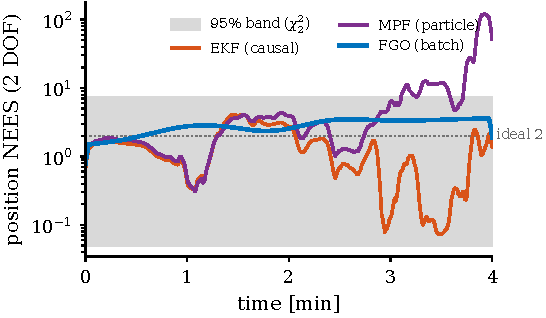
\includegraphics[width=0.98\columnwidth]{figs/fig_consistency.pdf}
\caption{Monte-Carlo position NEES versus time (EKF, marginalized particle filter,
and batch FGO) with the \SI{95}{\percent} $\chi^2_2$ band (ideal \num{2}, dotted).
NEES divides each estimator's error by its own reported covariance, so a
lower curve means a more conservative filter, not a more accurate one; the EKF's
larger errors over its larger causal covariance can plot below the more accurate
smoother. Accuracy is compared by DRMS in the text.}
\label{fig:consistency}
\end{figure}

\begin{figure}[t]
\centering
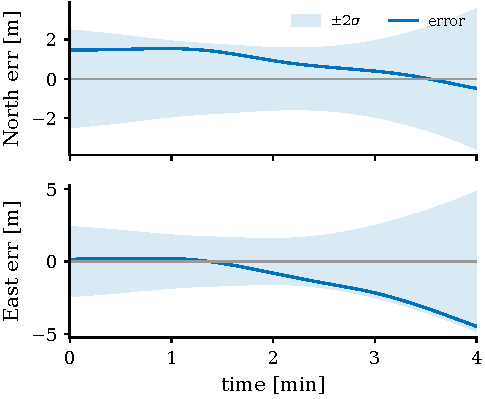
\includegraphics[width=0.98\columnwidth]{figs/fig_sigma.pdf}
\caption{North and East position error within the estimator $\pm2\sigma$ bands
(representative simulated run of the batch FGO; the envelope is the smoother's own
reported uncertainty, so this checks credibility, not accuracy). A calibrated
Gaussian $\pm2\sigma$ band would be exceeded on ${\approx}5\%$ of epochs per axis;
here the error approaches but never exits the band, the mildly conservative
behaviour consistent with the ANEES below \num{2}.}
\label{fig:sigma}
\end{figure}

\subsection{Cross-implementation validation}
Because every number above comes from our own code, a fair question is whether the
advantage belongs to the estimator or to one implementation. To separate the two, we
reran the primary line 1007.06 through a second, independent estimator: a Python
factor graph built on the GTSAM library~\cite{dellaert2012}, with its own
Levenberg--Marquardt and iSAM2 solvers, sharing no code with the in-house Julia
smoother, whose back end is an iterated Rauch--Tung--Striebel and Gauss--Newton pass.
Both solve the same factor graph of Section~\ref{sec:method} from the same inputs. We
first checked the port itself: the state-transition slices $\boldsymbol{\Phi}_t$, the
regressor rows $\mathbf{A}_t$, the scalar measurements, and the INS mechanization match
to the bit across the two languages, and the interpolated anomaly-map grid agrees to a
\SI{0.9}{\nano\tesla} standard deviation, so the two estimators see the same problem.

On the full \SI{87}{\minute} cold-start line, the two land within a metre of each
other: the GTSAM window returns \SI{12.4}{\meter} horizontal DRMS against the Julia
smoother's \SI{13.1}{\meter} under the marginalized handoff both use
(Table~\ref{tab:breadth}; the legacy smoothed handoff gives \SI{13.8}{\meter}), and on the first ten-minute
segment \num{17.5} against \SI{21.4}{\meter}, the GTSAM side being slightly the better of
the two in both cases; the free-inertial drift matches at \num{317.5} against
\SI{318}{\meter}, a further check that the two share the same trajectory and map. The
residual differences trace to modeling choices left deliberately independent:
Levenberg--Marquardt versus plain Gauss--Newton, bicubic versus bilinear map
interpolation, and a slightly different window handoff. The comparison covers one
line and each side is a single run, so this is a statement about implementation
independence rather than a statistical one; its value is that the bounded cold-start
result survives a complete change of language, library, and solver.
Fig.~\ref{fig:crossimpl} overlays the GTSAM error trace on the segment.

On the cabin magnetometer with the larger platform field the agreement is
conditional, and what it is conditional on is instructive. Run on Mag~4 of the
same line from a zero compensation, the GTSAM window returns \SI{5430}{\meter}
against the Julia smoother's \SI{30.7}{\meter}, with identical inputs and the
identical prior; on 1003.02 Mag~4 it returns \SI{36.6}{\meter} against
\SI{43.1}{\meter} and there is no discrepancy at all. The full-line GTSAM batch on
1007.06 Mag~4 returns \SI{18.6}{\meter}, so neither the graph nor its cost
function is at fault. Seeding the first window's compensation with the ridge fit
of Section~\ref{sec:window1}, which changes nothing else, brings the GTSAM
window on that case to \SI{30.8}{\meter} against the Julia smoother's
\SI{30.7}{\meter}. The two implementations therefore agree on both magnetometers
once the compensation cold start is handled, and the earlier disagreement was
where the first window's compensation started, not the language, the library, or
the solver. That the two behave differently from the same start is consistent
with the sensitivity of Section~\ref{sec:coldprior}: the Julia smoother stops
after at most five Gauss--Newton passes per window while the GTSAM window runs
Levenberg--Marquardt to convergence, so they sample that sensitivity differently.
We report that as the difference we observe, not as a mechanism we have isolated.

\begin{figure}[t]
\centering
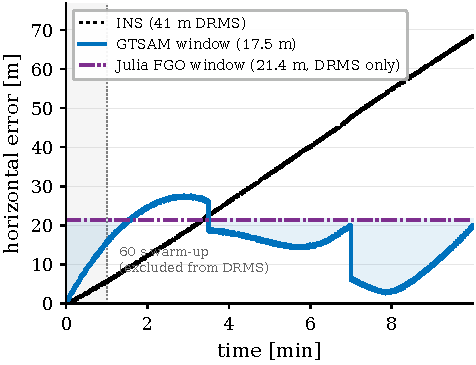
\includegraphics[width=\columnwidth]{figs/fig_crossimpl.pdf}
\caption{Horizontal error of the independent GTSAM sliding window on the first
ten-minute segment of line 1007.06, with the Julia smoother's segment DRMS shown as
a reference level (no Julia time series was exported for this run).}
\label{fig:crossimpl}
\end{figure}

\subsection{Real-time incremental smoothing}
Each window is a sparse nonlinear least-squares problem of fixed size
$O\big(L_w(n+m)\big)$; the block-bidiagonal Jacobian of the two chains
(Fig.~\ref{fig:graph}) is factored in $O(L_w)$ by the square-root
solver~\cite{dellaert2006}, and the number of Gauss--Newton iterations is small
(typically $3$--$5$) because the problem is mildly nonlinear away from observability
collapse. The per-window cost is therefore constant in the line length and the
overall complexity is linear in the number of epochs, matching a filter's
asymptotic cost while retaining the look-ahead. Memory is bounded by the window,
not the flight. The one-time overhead relative to an EKF is the window
factorization and the IRLS reweighting, which in our unoptimized research
implementation runs comfortably faster than real time on the SGL sampling rate.

\subsection{The compensation prior at cold start}\label{sec:coldprior}
Taken to its per-epoch limit, the smoother exposes a modeling choice that the
full-line batch tolerates. Run from a zero compensation on the cabin
magnetometer with the larger platform field (Mag~4), the incremental smoother at
a \SI{300}{\second} lag leaves the map on four of the five lines, three of the
four counted ones, and ends between \num{6.6} and \SI{27}{\kilo\meter} from
truth, while the same smoother on Mag~5 of the same flights navigates normally
(Table~\ref{tab:incprior}, first column). The asymmetry is the clue, and it is
one of magnitude. Over the first \SI{300}{\second}, the residual against the map
at the INS position is \SIrange{1729}{2081}{\nano\tesla} root-mean-square on
Mag~4 and \SIrange{22}{314}{\nano\tesla} on Mag~5, and the compensation
coefficients that explain the Mag~4 field have magnitudes of
\numrange{552}{722} in the units of Appendix~\ref{app:tl}.

Against that, the priors the model offers for anything other than position are
small. The compensation prior is $\mathbf{P}_0^{\beta}=\mathbf{I}(\sigma_{\beta})^2$
with $\sigma_{\beta}=1$, one scalar shared by all \num{19} coefficients, and the
FOGM disturbance prior is \SI{3}{\nano\tesla}. A cold start on Mag~4 therefore
presents the graph with roughly \SI{2000}{\nano\tesla} while both nuisance
channels are stiff, and the degree of freedom that is not stiff is position,
through the map gradient. The single shared
$\sigma_{\beta}$ is the weaker part of that: by Appendix~\ref{app:tl} the
regressor columns range over four orders of magnitude, from direction cosines of
order one to induced and eddy terms carrying the field magnitude, so no single
coefficient scale can be right for all of them.

Table~\ref{tab:priorsweep} measures the sensitivity. Widening $\sigma_{\beta}$
with the prior mean left at zero and nothing else changed removes the divergence
on every Mag~4 line: $\sigma_{\beta}=10$ already suffices and
\numrange{100}{1000} changes the result by up to \SI{14}{\meter}. We recommend
$\sigma_{\beta}=100$ and use it for the rest of this subsection: the Mag~4 lines
settle at \num{19.6}, \num{25.0}, \num{99.1}, \num{28.4} and
\SI{24.2}{\meter} and the Mag~5 lines at \num{12.0}, \num{10.5}, \num{101.0},
\num{15.8} and \SI{11.5}{\meter}. A per-column prior, one that assigns each basis
column a standard deviation of \SI{100}{\nano\tesla} of measurement contribution
instead of a common coefficient scale, is the dimensionally consistent version of
the same change and performs the same to within the line-to-line spread
(Table~\ref{tab:priorsweep}). It does not, however, keep the coefficients
smaller: after warm-up the median of $\|\boldsymbol{\beta}\|_\infty$ is
\numrange{787}{1167} across the Mag~4 lines at $\sigma_{\beta}=100$ and
\numrange{2485}{5995} under the per-column prior, against the
\numrange{552}{722} that a ridge fit of the same data needs. Any prior loose
enough to fix the cold start also lets the compensation basis absorb model error
beyond the platform field, and we report that as a cost of the setting rather
than a property we have controlled. Widening the FOGM disturbance prior and
walk instead, leaving the compensation prior nominal, recovers three of the five
lines at a factor of \num{10} and four at a factor of \num{100}, leaving 1006.08
diverged in both cases (Table~\ref{tab:priorsweep}), so the effect is not specific to the compensation
block, although the compensation basis is where the interference belongs.

We do not claim more than the sensitivity we measured. In particular the
mechanism is not simply that the coefficients cannot reach the platform field:
the window solves of Section~\ref{sec:window1} reach $\|\boldsymbol{\beta}\|_\infty$
of \numrange{463}{795} across lines at $W\ge\SI{100}{\second}$ even at
$\sigma_{\beta}=1$, and the prior term at that
magnitude is outweighed by the measurement term by more than two orders of
magnitude. What the tight, dimensionally inconsistent prior does is stiffen the
first linearizations in $\boldsymbol{\beta}$ relative to position, and the
per-epoch smoother commits and marginalizes states while that is true.

Seven alternatives can be dismissed by measurement, all at the nominal prior on
line 1007.06 Mag~4 against its \SI{19.5}{\kilo\meter} unless stated. The robust
kernel is not sufficient to explain the failure: removing it entirely gives
\SI{33.0}{\kilo\meter}, and widening the Huber constant from \num{1.345} to
\num{10} and \num{100} gives \num{18.0} and \SI{33.0}{\kilo\meter}, while Mag~5
of the same line returns \SI{11.7}{\meter} with the kernel and \SI{11.7}{\meter}
without it. Map resolution is not sufficient: re-exporting the anomaly grid at
\SI{34}{\meter} spacing instead of \SI{113}{\meter} gives \SI{13.7}{\kilo\meter}.
The lag is not sufficient: at $\sigma_{\beta}=1$, lags of \num{300},
\num{450}, \num{600} and \SI{900}{\second} give \num{19.5}, \num{14.8},
\num{14.7} and \SI{14.5}{\kilo\meter}. Retained linearization is not
sufficient: relinearizing every variable at every update gives
\SI{9.8}{\kilo\meter}. Measurement thinning is not the cause: attaching all ten
raw samples to their nearest kept state gives \SI{22.9}{\kilo\meter}. Nor is the
measurement noise, which is the alternative worth taking most seriously because
the compensated residual on Mag~4 is several times the assumed
$\sqrt{R}=\SI{12}{\nano\tesla}$: no single value of $\sqrt{R}$ repairs
it across lines. Setting it to \SI{150}{\nano\tesla} recovers 1007.06 to
\SI{64.5}{\meter} and leaves 1003.02 at \SI{31}{\kilo\meter}; setting it to
\SI{65}{\nano\tesla} recovers 1007.02 to \SI{41.8}{\meter} and leaves 1007.06
at \SI{7.3}{\kilo\meter}. Across the ten runs the result ranges from
\SI{42}{\meter} to \SI{46}{\kilo\meter} with no setting bounded everywhere,
where raising $\sigma_{\beta}$ is bounded on every line at once. The
$10^{-20}$ conditioning floor on the process noise is likewise not doing the
work: raising it to $10^{-16}$ gives \SI{49}{\kilo\meter} and lowering it to
$10^{-24}$ gives \SI{12.9}{\kilo\meter}. Each of these moves the number and none
recovers the solution, which is what separates a contributing factor from the
one setting that does.

Two measurements bound how far the modeling error reaches. The same graph for
line 1007.06 Mag~4, solved as one full-line batch from the same zero start and
the same nominal prior, reaches \SI{18.6}{\meter}: over a whole line the
compensation has time to move and the map has gradient enough to hold position,
so the cost function itself is sound and the sensitivity is a property of short
spans. The sliding window of Section~\ref{sec:window}, run in this same code
base, sits between the two. At the nominal prior it diverges on 1007.06 Mag~4
(\SI{5430}{\meter}) but not on 1003.02 Mag~4 (\SI{36.6}{\meter}), and seeding its
first window with a ridge fit of the compensation brings 1007.06 to
\SI{30.8}{\meter}, which is the cross-implementation comparison of
Section~\ref{sec:results}-F. The sensitivity is therefore not peculiar to
per-epoch marginalization; it grows as the span each solve sees gets shorter.

A caveat on the divergent runs themselves. The exported anomaly grid covers the
trajectory with a \SI{2.2}{\kilo\meter} margin, and the interpolator clamps
outside it, so once an estimate leaves the grid the map gradient vanishes and no
information can pull it back. The kilometre-scale numbers in the first column of
Table~\ref{tab:incprior} are therefore a floor on how bad the divergence is, not
a measurement of where an unclamped estimator would have gone; what they
establish is that the estimate left the map, not how far.

\begin{figure}[t]
\centering
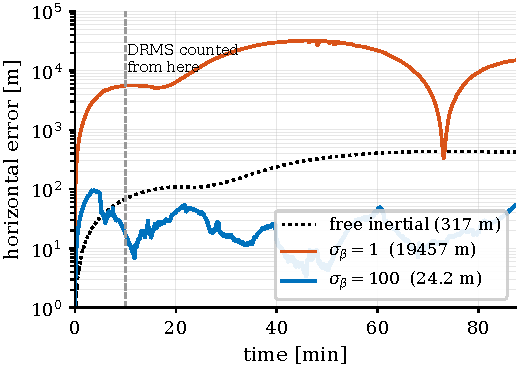
\includegraphics[width=\columnwidth]{figs/fig_prior.pdf}
\caption{Per-epoch smoother on line 1007.06 Mag~4 at a \SI{300}{\second} lag. At
the nominal compensation prior the estimate leaves the map in the first minutes
and never returns; with the compensation prior raised to $\sigma_{\beta}=100$, and nothing else
changed, it stays an order of magnitude below free-inertial drift for the whole
line.}
\label{fig:prior}
\end{figure}

\subsection{The same prior, seen in a single window}\label{sec:window1}
The explanation can be tested one window at a time, which also answers how much
flight the joint problem needs before it is determined. Table~\ref{tab:knee}
reports the solution reached when the same graph is solved as a batch over only
its first $W$ seconds, from a zero compensation, at both priors, with no
commitment and no marginalization anywhere. At $\sigma_{\beta}=1$, the Mag~4
solutions pass through a region, covering at least \SIrange{100}{200}{\second} on
all five lines and extending to \SI{400}{\second} on 1007.06, in which they sit
hundreds of metres to kilometres from truth, while Mag~5 stays within tens of
metres except on the short line 1006.08. At $\sigma_{\beta}=1000$, that region is
gone: every Mag~4 entry outside 1006.08 falls between \num{2} and
\SI{125}{\meter}, and line 1007.02 Mag~4, which at the tight prior never left the
region within the sweep, is at or below \SI{94}{\meter} at every window length.
The single-window and the full-line experiments therefore agree, and they turn on
the same parameter (Fig.~\ref{fig:knee}).

This also fixes what the failure needs. It is not early commitment: these window
solves commit nothing and still land kilometres out. It is a short data span
together with a prior that is not scaled to the regressor. Marginalization only
decides whether the estimator can recover afterwards, and in the fixed-lag case
it cannot.

Line 1006.08 is the exception at both priors. It stays at hundreds of metres
across its middle window lengths and improves only slowly, which is consistent
with the low map-information floor of Remark~\ref{rem:floor} rather than with the
compensation: where $\mathbf{G}\!\approx\!\mathbf{0}$, no prior on
$\boldsymbol{\beta}$ can help.

\begin{figure}[t]
\centering
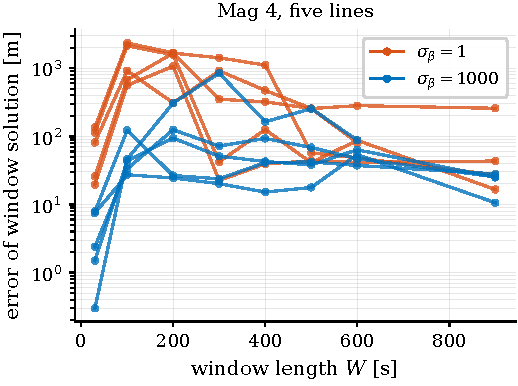
\includegraphics[width=\columnwidth]{figs/fig_knee.pdf}
\caption{Position error of the batch solution over the first $W$ seconds of each
Mag~4 line, from a zero compensation. At the nominal prior the solutions climb to
kilometres over the middle window lengths; at the widened prior the excursion is
absent on every line but the short calibration line 1006.08.}
\label{fig:knee}
\end{figure}

One negative result belongs here because we specifically tested for it. We also
repeated the sweep from a compensation seeded with a ridge fit of
$(z_t-h(\mathbf{p}^{\mathrm{ins}}_t))$ over the same $W$ seconds, to test whether
the far-from-truth solutions are a matter of which minimum the solver selects.
Across the \num{78} combinations of line, magnetometer, and $W$, the two starts
reach objectives that differ at all in only \num{7}; of those, the seeded start
is the cheaper and the more accurate one in \num{5}, and in \num{2} the cheaper
solution is the less accurate one. The window solve is largely indifferent to
where it starts. We therefore do not attribute the cold-start failure to minimum
selection, and we do not claim that the accurate solution can be identified
online by comparing objective values.

\subsection{Real-time cost}\label{sec:realtime2}
With the compensation prior raised to $\sigma_{\beta}=100$, the per-epoch smoother runs
the full breadth at a \SI{300}{\second} lag. Graph states are placed at
\SI{1}{\hertz} rather than at the \SI{10}{\hertz} sample rate, with the
transition compounded and the process noise accumulated exactly over the ten
intervening samples, so the \SI{300}{\second} lag is a \num{300}-state window
updated once a second. Across the ten cases, the update takes
\SIrange{6.0}{9.0}{\milli\second} per state, mean \SI{7.8}{\milli\second}, so an
\SI{87}{\minute} line finishes in \SI{42}{\second} and the margin against the
\SI{1}{\hertz} state cadence is two orders of magnitude. These are mean times on
one core of a laptop-class x86 processor under WSL2, with the measurement factor
evaluated through a Python callback, so they are an upper bound on what native
factors would cost; the corresponding costs in the
relinearization and dense-measurement runs are \SI{75.5}{\milli\second} per
state with every variable relinearized at every update and
\SIrange{28.7}{35.1}{\milli\second} with all ten raw measurements attached.
Placing states at the full \SI{10}{\hertz} instead makes the same lag a
\num{3000}-state window, which is why a \SI{300}{\second} lag is reported here at
\SI{1}{\hertz} states and not at the sample rate.

The decimation costs the nine measurements dropped between kept states, and on
these lines it does not cost accuracy. The aircraft covers \SI{68}{\meter} per
kept state at the survey ground speed. Attaching all ten raw samples to their
nearest kept state instead of one returns \SI{26.7}{\meter} against
\SI{23.9}{\meter} on line 1007.06 Mag~4 and \SI{26.2}{\meter} against
\SI{19.2}{\meter} on 1003.02 Mag~4, both pairs run with the ridge-seeded cold
start rather than the widened prior because that is the pair we have, for \numrange{3.5}{3.8} times the
computation. Two things are folded into that comparison and we can separate
neither with the runs we have: the dense variant attaches all ten factors to one
state, so it also assumes a single error state over the \SI{1}{\second} span, and
the measurements themselves are unlikely to be independent at \SI{10}{\hertz}
given that the compensated residual on these lines is several times $\sqrt{R}$. We
report the comparison as a reason not to treat the decimation as a pure loss, not
as evidence about the noise model, which would need an innovation whiteness test
we have not run on these lines.

\begin{table}[t]
\caption{Per-epoch incremental smoother, \SI{300}{\second} lag, \SI{1}{\hertz}
states, at the nominal compensation prior and at the recommended one. Smoothed DRMS [m]
after a \SI{600}{\second} warm-up, causal value in parentheses; DRMS is evaluated
at the \SI{1}{\hertz} state grid, and INS is the free-inertial drift computed on
the same grid by the same code. ``div.''\ $>\SI{1}{\kilo\meter}$ and, given the
grid clamping discussed in the text, is a lower bound. Line 1006.08 is the
\SI{14}{\minute} calibration line set aside in Section~\ref{sec:results}; on its
Mag~5 the smoothed estimate is worse than the causal one at both priors, which we
read with Remark~\ref{rem:floor} as the map-information floor rather than as a
smoothing gain.}
\label{tab:incprior}
\centering
\setlength{\tabcolsep}{4pt}
\begin{tabular}{llr rr}
\toprule
Line & Mag & INS & $\sigma_{\beta}=1$ & $\sigma_{\beta}=100$ \\
\midrule
1003.02 & 4 & 123.8 & div. & \textbf{19.6} (58.2) \\
1003.02 & 5 & 123.8 & 12.6 (24.4) & 12.0 (21.9) \\
1003.08 & 4 & 271.9 & div. & \textbf{25.0} (48.9) \\
1003.08 & 5 & 271.9 & 10.9 (22.4) & 10.5 (19.2) \\
1006.08 & 4 & 197.7 & div. & \textbf{99.1} (134.8) \\
1006.08 & 5 & 197.7 & 83.9 (52.4) & 101.0 (80.1) \\
1007.02 & 4 & 120.7 & 60.0 (327.8) & \textbf{28.4} (74.3) \\
1007.02 & 5 & 120.7 & 14.0 (40.3) & 15.8 (33.1) \\
1007.06 & 4 & 317.5 & div. & \textbf{24.2} (42.7) \\
1007.06 & 5 & 317.5 & 11.7 (19.8) & 11.5 (16.0) \\
\bottomrule
\end{tabular}
\end{table}

\begin{table}[t]
\caption{Prior sweep on the Mag~4 lines, zero prior mean, no other change:
smoothed DRMS [m] after a \SI{600}{\second} warm-up. The first four columns scale
the single shared coefficient standard deviation $\sigma_{\beta}$; ``per col.''\
instead gives every regressor column a prior of \SI{100}{\nano\tesla} of
measurement contribution; ``$\sigma_S$''\ leaves the compensation prior at
nominal and widens the FOGM disturbance prior and walk a hundredfold instead.}
\label{tab:priorsweep}
\centering
\setlength{\tabcolsep}{4pt}
\begin{tabular}{l rrrr rr}
\toprule
 & \multicolumn{4}{c}{$\sigma_{\beta}$} & per col. & $\sigma_S$ \\
\cmidrule(lr){2-5}
Line & 1 & 10 & 100 & 1000 & 100 nT & $\times100$ \\
\midrule
1003.02 & 26810 & 32.7 & 19.6 & 19.3 & \textbf{19.0} & 33.2 \\
1003.08 & 11262 & 25.7 & 25.0 & 24.5 & \textbf{25.1} & 29.8 \\
1006.08 & 6574 & 117.7 & 99.1 & 85.4 & \textbf{98.9} & 1144 \\
1007.02 & 60.0 & 30.3 & 28.4 & 30.3 & \textbf{30.5} & 56.7 \\
1007.06 & 19457 & 24.1 & 24.2 & 23.9 & \textbf{23.7} & 27.3 \\
\bottomrule
\end{tabular}
\end{table}

\begin{table}[t]
\caption{Solution reached by Levenberg--Marquardt from a zero compensation on a
batch over only the first $W$ seconds of each line: horizontal DRMS [m] over
those $W$ seconds, at the nominal and at a uniformly widened compensation prior.
These are the solutions the solver reaches, not certified global optima. The
free-inertial drift over the same spans runs from \SIrange{0.4}{5.0}{\meter} at
$W=\SI{30}{\second}$ to \SIrange{56.5}{100.7}{\meter} at $W=\SI{900}{\second}$,
so an entry below about \SI{100}{\meter} is at or under the drift it has to beat.}
\label{tab:knee}
\centering
\setlength{\tabcolsep}{3pt}
\begin{tabular}{ll c rrrrrrrr}
\toprule
 & & & \multicolumn{8}{c}{$W$ [s]} \\
\cmidrule(l){4-11}
Line & Mag & $\sigma_{\beta}$ & 30 & 100 & 200 & 300 & 400 & 500 & 600 & 900 \\
\midrule
1003.02 & 4 & 1 & 113 & 2137 & 1569 & 42 & 126 & 41 & 87 & 17 \\
        &   & 1000 & 8 & 27 & 24 & 20 & 15 & 18 & 54 & 11 \\
1003.02 & 5 & 1 & 11 & 42 & 13 & 10 & 9 & 24 & 8 & 11 \\
        &   & 1000 & 12 & 55 & 11 & 12 & 11 & 14 & 16 & 11 \\
1003.08 & 4 & 1 & 20 & 558 & 1069 & 23 & 39 & 44 & 42 & 43 \\
        &   & 1000 & 8 & 123 & 27 & 24 & 41 & 42 & 37 & 28 \\
1003.08 & 5 & 1 & 26 & 70 & 14 & 12 & 24 & 20 & 24 & 22 \\
        &   & 1000 & 3 & 18 & 11 & 3 & 12 & 15 & 11 & 10 \\
1006.08 & 4 & 1 & 81 & 917 & 310 & 915 & 472 & 257 & 81 & -- \\
        &   & 1000 & $<$1 & 46 & 308 & 847 & 164 & 255 & 88 & -- \\
1006.08 & 5 & 1 & 48 & 136 & 341 & 70 & 115 & 50 & 36 & -- \\
        &   & 1000 & 6 & 67 & 113 & 35 & 81 & 26 & 31 & -- \\
1007.02 & 4 & 1 & 136 & 2344 & 1676 & 350 & 321 & 256 & 282 & 258 \\
        &   & 1000 & 2 & 43 & 94 & 51 & 43 & 38 & 63 & 25 \\
1007.02 & 5 & 1 & 13 & 15 & 32 & 34 & 44 & 34 & 60 & 34 \\
        &   & 1000 & 3 & 18 & 22 & 23 & 41 & 37 & 66 & 35 \\
1007.06 & 4 & 1 & 26 & 676 & 1662 & 1420 & 1109 & 57 & 48 & 27 \\
        &   & 1000 & 2 & 33 & 125 & 72 & 93 & 68 & 47 & 25 \\
1007.06 & 5 & 1 & 23 & 78 & 90 & 20 & 17 & 19 & 19 & 12 \\
        &   & 1000 & 1 & 8 & 26 & 11 & 13 & 12 & 10 & 7 \\
\bottomrule
\end{tabular}
\end{table}

These same properties make the estimator compatible with online, fixed-lag
operation rather than zero-latency filtering. Its committed output lags real time by
the overlap $L_o$, here \SI{90}{\second}, a latency that suits the map-aiding role,
in which the INS supplies the high-rate real-time solution and the smoother corrects
it periodically at the commit cadence ($L_w-L_o$, here \SI{3.5}{\minute}), and that
the designer trades against accuracy through $L_o$. The factor interface is modular, so
compensation and map factors can be added or removed without touching
the solver, and one implementation then covers both the calibrated case with frozen
coefficients and the cold-start case with adaptive coefficients. Integrating it with an operational system amounts to feeding
the INS mechanization, fluxgate, and scalar magnetometer streams into the graph and
reading back the corrected position at the commit rate. The main tuning burden is
the two window parameters and the compensation process noise $\mathbf{Q}^{\beta}$,
all of which have clear physical meaning.

\section{Conclusion}\label{sec:conclusion}
This paper formulated airborne magnetic-anomaly navigation as factor-graph MAP
estimation and used the formulation to solve the cold-start compensation problem
jointly with navigation. The Tolles--Lawson coefficients enter the graph as
time-varying variables, so the compensation adapts along the flight and
late-arriving calibration information corrects early navigation states, the
mechanism a one-pass causal filter lacks; and a linear condition states when
position and compensation can be separated at all. That single MAP problem is
realized across a lag spectrum, from a full-line batch that fixes the offline
accuracy bound, through a fixed-lag window, to a per-epoch incremental smoother that
runs a \SI{300}{\second} lag in real time at
\SIrange{6.0}{9.0}{\milli\second} per state. On real SGL~2020 data the
per-epoch estimator stays bounded from a cold start on all eight full-length
cabin-magnetometer cases, where the plain online-TL EKF diverges and a marginalized
particle filter is erratic, and it is more accurate on every such case than the
tuned online EKF+TL+NN baseline, with no neural network and no calibration flight. A Monte-Carlo
simulation shows its reported covariance is consistent and conservative
where the toolbox particle filter's is over-confident; the recorded platform
currents confirm the absorption mechanism, explaining a third of the raw cabin
interference but almost none of the post-fit residual; and an independent GTSAM
reimplementation that shares no code reproduces the bounded cold-start result,
separating the estimator from its implementation.

Several limitations bound the study. Each real line is a single physical
realization, so its DRMS is a point estimate, and the cross-implementation check is
likewise a single run that establishes implementation independence rather than a
statistical claim; distributional statements come from the Monte-Carlo simulation
only. The baseline set, though it now spans a weak causal filter, the strongest
reported causal method, and a particle filter, still lacks a grid or point-mass MMSE
map-matcher~\cite{bergman1999,nordlund2009}. The compensation basis is
attitude-only: physically structured sensor-error states (heading harmonics, dead
zones) and direct regression of current telemetry are natural graph extensions, but
our exploratory tests show that applying either blindly, without documented sensor
hardware and orientation, or with na\"{\i}vely scaled telemetry, can help or hurt by
tens of percent depending on the line, so neither is claimed here. The warm-start
prior used above is drawn from the same line rather than transferred from a separate
calibration flight, so a true cross-line warm start remains untested, and the
observability gate the separability condition suggests is analyzed but not yet
folded into the online estimator. The per-epoch smoother reaches a
\SI{300}{\second} lag in real time only by placing states at \SI{1}{\hertz}; at the
full \SI{10}{\hertz} state cadence, that lag is a window ten times as large and
remains offline in this implementation, a limit we expect native factors to lift.
The compensation prior the cold start needs is a measured setting, not a derived
one: a shared $\sigma_{\beta}=1$ is far too tight, anything from \num{10} to
\num{1000} works on these installations, and a dimensionally consistent
per-column prior works equally well, but we give no rule for choosing the scale
from installation data, and no setting we found both fixes the cold start and
holds the coefficients at the magnitude a direct fit of the same data needs. A related limit bounds the comparison itself. The window and
filter results of Section~\ref{sec:results} were produced at the nominal prior. The window smoother is bounded there on every
counted case, so its numbers are not themselves an artifact of the prior, though
the independent GTSAM window diverges on 1007.06 Mag~4 at that same prior
(Section~\ref{sec:results}-F), so the boundedness is not robust across
implementations. We have not re-run either the window or the causal EKF baselines
at a corrected prior. Part of the EKF cold-start divergence on the cabin magnetometers may
therefore be the same modeling effect rather than a property of causal filtering,
and the margin the window shows over those baselines is an upper bound on the
margin that survives a corrected prior. And none of
the SGL~2020 lines is a long, straight-and-level operational transit: the attitude
content that stresses compensation also excites the TL regressor and aids its
observability, so performance under the weak excitation of a pure cruise is not
established here. Short lines remain hard for every method, an information limit
rather than an estimator one.

These limitations set the agenda for further work: extending the evaluation to the
full SGL line set and a grid or point-mass baseline; lag scheduling that runs a long
lag through the early, weakly observable minutes and contracts once the compensation
has converged, moved online by native factors; transferring a compensation prior
across lines for a true warm start; folding the separability condition into an
online observability gate; making the sensor-error and current-telemetry extensions
robust enough to claim, both staying within the attitude-derived,
position-independent basis the condition requires; and testing a low-excitation
operational cruise. None of these qualifications affects the central and reproducible
finding: carrying the compensation as time-varying variables of a windowed factor
graph, solved anywhere along the lag spectrum, is sufficient to survive the cold
start and to match or beat an NN-augmented causal filter on this benchmark, with
every estimated quantity a physically interpretable state.

\appendices
\section{Pinson Error-State Dynamics}\label{app:pinson}
The navigation-error block of $\boldsymbol{\Phi}_t$ in~\eqref{eq:dyn} follows the
Pinson model in a local north-east-down frame~\cite{titterton2004,groves2013}. With
position, velocity, and attitude errors $(\delta\mathbf{p},\delta\mathbf{v},
\boldsymbol{\psi})$ and sensor biases $(\mathbf{b}_a,\mathbf{b}_g)$, the continuous
error dynamics are
\begin{equation}
\begin{aligned}
\dot{\delta\mathbf{p}}&=\mathbf{F}_{pp}\,\delta\mathbf{p}+\delta\mathbf{v},\\
\dot{\delta\mathbf{v}}&=\mathbf{F}_{vp}\,\delta\mathbf{p}
+\mathbf{F}_{vv}\,\delta\mathbf{v}
-[\mathbf{f}^n\times]\,\boldsymbol{\psi}+\mathbf{C}^n_b\mathbf{b}_a,\\
\dot{\boldsymbol{\psi}}&=\mathbf{F}_{\psi p}\,\delta\mathbf{p}
+\mathbf{F}_{\psi v}\,\delta\mathbf{v}
-[\boldsymbol{\omega}^n_{in}\times]\,\boldsymbol{\psi}-\mathbf{C}^n_b\mathbf{b}_g,
\end{aligned}
\label{eq:pinson}
\end{equation}
where $\mathbf{f}^n$ is the specific force, $\mathbf{C}^n_b$ the body-to-nav rotation,
$\boldsymbol{\omega}^n_{in}$ the inertial rate, $[\cdot\times]$ the skew operator, and
the $\mathbf{F}_{\bullet\bullet}$ blocks collect the transport-rate, gravity-gradient,
and Coriolis terms. The biases follow first-order Gauss--Markov or random-walk models,
as does the scalar magnetic disturbance state $S$ with correlation time $\tau$. The
discrete $\boldsymbol{\Phi}_t=\exp(\mathbf{F}_t\,\Delta t)$ and $\mathbf{Q}_t$ are
obtained by standard van~Loan discretization~\cite{farrell2008}. Only
$\mathbf{g}_t^{\top}$, the position row of the measurement Jacobian~\eqref{eq:jac},
couples this block to the map.

\section{Tolles--Lawson Basis}\label{app:tl}
The basis row $\mathbf{A}_t$ of~\eqref{eq:tlbasis} is built from the fluxgate
direction cosines $\hat{\mathbf{b}}=[\,u\;v\;w\,]^{\top}$ (with $u^2+v^2+w^2=1$) and
the scalar field magnitude $B$~\cite{tolles1950,leliak1961}. The permanent moment
contributes the three cosines $(u,v,w)$; the induced magnetization, symmetric in the
field, contributes the six products
$B\,(u^2,uv,uw,v^2,vw,w^2)$; and the eddy-current field, proportional to the rate of
change of the cosines, contributes the nine products $B\,(u\dot u,u\dot v,\dots,
w\dot w)$. Stacking these gives an eighteen-term basis, optionally augmented by a
constant bias, and $c_t=\mathbf{A}_t^{\top}\boldsymbol{\beta}_t$ is linear in the
coefficients $\boldsymbol{\beta}_t$, the property that lets them enter the factor
graph as ordinary linear-measurement variables. In the cold-start regime the
calibration flight that classically fixes $\boldsymbol{\beta}$ is unavailable, which
is precisely why we carry it as a graph variable.

\section*{Acknowledgment}
The experiments use the publicly released SGL~2020 challenge
dataset~\cite{gnadt2020}.

\begin{biography}[{
\includegraphics[width=1in,height=1.25in,clip,keepaspectratio]{figs/author_lee.png}}]{Jayden Dongwoo Lee}
received the M.S. degree in aerospace engineering from the Korea Advanced Institute
of Science and Technology (KAIST), Daejeon, South Korea, in 2021. He is currently
pursuing the Ph.D. degree in aerospace engineering at KAIST. His research interests
include unmanned aircraft systems (UAS), guidance and navigation, adaptive and
data-driven control, and estimation.
\end{biography}

\begin{biography}[{
\includegraphics[width=1in,height=1.25in,clip,keepaspectratio]{figs/author_placeholder.png}}]{Bohyun Chang}
is with the Department of Aerospace Engineering, Korea Advanced Institute of Science
and Technology (KAIST), Daejeon, South Korea. His research interests include
guidance, navigation, and control of aerospace vehicles. (Detailed biography to be
provided by the author.)
\end{biography}

\begin{biography}[{
\includegraphics[width=1in,height=1.25in,clip,keepaspectratio]{figs/author_bang.jpg}}]{Hyochoong Bang}
received his Ph.D. degree in aerospace engineering from Texas
A\&M University in 1992. Since 2001, he has been with the Department of Aerospace
Engineering, Korea Advanced Institute of Science and Technology (KAIST), Daejeon,
South Korea, as a professor. His research interests include spacecraft guidance,
attitude dynamics and control, unmanned aerial vehicle flight dynamics and control,
and flight control system design.
\end{biography}

\section{Proof of Proposition~\ref{prop:obs}}\label{app:proof}
Two joint states $(\delta\mathbf{p},\delta\boldsymbol{\beta})$ and
$(\delta\mathbf{p}',\delta\boldsymbol{\beta}')$ produce identical noise-free
predictions iff
$\mathbf{G}(\delta\mathbf{p}-\delta\mathbf{p}')=\boldsymbol{\Psi}(\delta\boldsymbol{\beta}'-\delta\boldsymbol{\beta})$,
i.e.\ iff
$[\,\mathbf{G}\;\;\boldsymbol{\Psi}\,]
[(\delta\mathbf{p}-\delta\mathbf{p}')^{\top}\;(\delta\boldsymbol{\beta}-\delta\boldsymbol{\beta}')^{\top}]^{\top}=\mathbf{0}$.
The unobservable subspace is therefore exactly
$\ker[\,\mathbf{G}\;\;\boldsymbol{\Psi}\,]$, and the joint state is observable iff
$[\,\mathbf{G}\;\;\boldsymbol{\Psi}\,]$ has full column rank; the first statement
of the proposition follows by taking $\delta\boldsymbol{\beta}'$ free and
$\delta\mathbf{p}'=\mathbf{0}$.

For the three-condition equivalence: if (i) fails, take
$\delta\mathbf{p}\in\ker\mathbf{G}\setminus\{\mathbf{0}\}$, giving the kernel
element $(\delta\mathbf{p},\mathbf{0})$; if (ii) fails, take
$\delta\boldsymbol{\beta}\in\ker\boldsymbol{\Psi}\setminus\{\mathbf{0}\}$, giving
$(\mathbf{0},\delta\boldsymbol{\beta})$; if (iii) fails, take
$\mathbf{G}\,\delta\mathbf{p}=\boldsymbol{\Psi}\,\delta\boldsymbol{\beta}\neq\mathbf{0}$,
giving $(\delta\mathbf{p},-\delta\boldsymbol{\beta})$. Conversely, let
$(\delta\mathbf{p},\delta\boldsymbol{\beta})\neq(\mathbf{0},\mathbf{0})$ lie in the
kernel, so $\mathbf{G}\,\delta\mathbf{p}=-\boldsymbol{\Psi}\,\delta\boldsymbol{\beta}$.
If $\mathbf{G}\,\delta\mathbf{p}=\mathbf{0}$ then either
$\delta\mathbf{p}\neq\mathbf{0}$ violates (i) or
$\delta\boldsymbol{\beta}\neq\mathbf{0}$ violates (ii); if
$\mathbf{G}\,\delta\mathbf{p}\neq\mathbf{0}$ it is a nonzero shared direction,
violating (iii). \hfill$\blacksquare$

\bibliographystyle{IEEEtaes}
\bibliography{references}

\end{document}
